% ****** Start of file apssamp.tex ******
%
%   This file is part of the APS files in the REVTeX 4.2 distribution.
%   Version 4.2a of REVTeX, December 2014
%
%   Copyright (c) 2014 The American Physical Society.
%
%   See the REVTeX 4 README file for restrictions and more information.
%
% TeX'ing this file requires that you have AMS-LaTeX 2.0 installed
% as well as the rest of the prerequisites for REVTeX 4.2
%
% See the REVTeX 4 README file
% It also requires running BibTeX. The commands are as follows:
%
%  1)  latex apssamp.tex
%  2)  bibtex apssamp
%  3)  latex apssamp.tex
%  4)  latex apssamp.tex
%
\documentclass[%
 reprint,
%superscriptaddress,
%groupedaddress,
%unsortedaddress,
%runinaddress,
%frontmatterverbose, 
%preprint,
%preprintnumbers,
%nofootinbib,
%nobibnotes,
%bibnotes,
 amsmath,amssymb,
 aps,
%pra,
prb,
%rmp,
%prstab,
%prstper,
%floatfix,
]{revtex4-2}

\usepackage{graphicx}% Include figure files
\usepackage{dcolumn}% Align table columns on decimal point
\usepackage{bm}% bold math
\usepackage{hyperref}% add hypertext capabilities
\hypersetup{colorlinks=true,urlcolor={blue},citecolor={blue}, linkcolor={blue}}
\usepackage{amsmath} % or simply amstext
%\newcommand{\angstrom}{\textup{\AA}}
\usepackage{siunitx}
\usepackage{color}
%\usepackage{url}            % simple URL typesetting
%\usepackage[mathlines]{lineno}% Enable numbering of text and display math
%\linenumbers\relax % Commence numbering lines
%\usepackage{nameref}

%\usepackage[showframe,%Uncomment any one of the following lines to test 
%%scale=0.7, marginratio={1:1, 2:3}, ignoreall,% default settings
%%text={7in,10in},centering,
%%margin=1.5in,
%%total={6.5in,8.75in}, top=1.2in, left=0.9in, includefoot,
%%height=10in,a5paper,hmargin={3cm,0.8in},
%]{geometry}

%RZK: do not edit red text
\newcommand{\lock}{\color{red}}

\begin{document}

\preprint{APS/123-QED}

\title{Adatoms in the surface Ullmann coupling}% Force line breaks with \\
%\thanks{A footnote to the article title}%

\author{Zhenzhe Zhang}
 %\altaffiliation[Also at ]{Physics Department, XYZ University.}%Lines break automatically or can be forced with \\
\author{Dmitrii F. Perepichka}%
 %\email{dmitrii.perepichka@mcgill.ca}
\author{Rustam Z. Khaliullin}
 %\email{rustam.khaliullin@mcgill.ca}
\affiliation{%
 Department of Chemistry, McGill University,\\ 801 Sherbrooke St West, Montreal, QC H3A 0B8, Canada
 %This line break forced with \textbackslash\textbackslash
}%

%\date{\today}% It is always \today, today,
             %  but any date may be explicitly specified

\begin{abstract}
This manuscript reviews the results of experimental and computational studies of the surface Ullmann coupling that shed light on the role of surface adatoms in its mechanism. A particular focus is on the early stages of the polymerization and coupling of two monomers.
\end{abstract}

\maketitle

%\tableofcontents

%RZK. What a variety of RZK labels mean. 
%R1111 or RZKmmdd - mm denotes month, dd - denotes day
%RZKX - these are low priority comments, which will be promoted to regular labels later 
%RZZK - can be ignored, these labels keep track of my own revision process

\section{Introduction}

{\lock

\subsection{Ullmann coupling in solution}

In 1901, Fritz Ullmann discovered~\cite{ullmann_01} a coupling reaction that \underline{creates a C--C bond between two aryl halides}
{\color{blue}
synthesized symmetric biphenyls from aryl halides
}
in the presence of a stoichiometric amount of Cu powder. 
%Currently, the scope of Ullmann coupling reaction is being widened with an increasing number of substrates, leaving groups, and active metal species being investigated for constructing various C--X bonds. 
Because of its ability to form C--C bonds, Ullmann coupling has become one of the key reactions in organic synthesis with its scope extended to new reactants and catalysts. 
Today, the \emph{classical} Ullmann or simply Ullmann reaction refers to a family of nucleophilic substitution reactions between aromatic nucleophiles that proceed in the presence of copper and lead to the formation of C--C and C--heteroatom bonds such as C--N~\cite{ullmann_02, ullmann_03}, C--O~\cite{ullmann_04}, C--S~\cite{ullmann_05} and C--P~\cite{ullmann_21,ullmann_22} bonds (Fig.~\ref{fig:UllmannCoupling}). 
%RZZK: In Ullmann coupling, metals can serve as reactants or as catalysts.

\begin{figure}[htb]
\centering
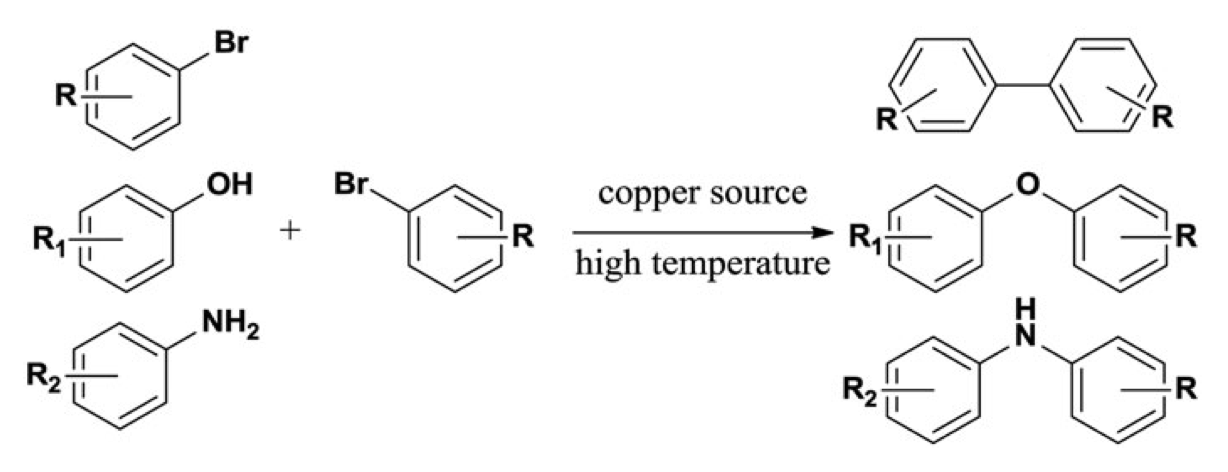
\includegraphics[width=0.90\columnwidth]{Fig/classical.png}
\caption{Examples of the Ullmann coupling reactions.}
\label{fig:UllmannCoupling}
\end{figure}

Depending on the type of bonds created, reactants in the Ullmann coupling can be aromatic amines~\cite{ullmann_17,ullmann_18}, amides~\cite{ullmann_19,ullmann_20}, phosphines~\cite{ullmann_21,ullmann_22}, carboxylic acids~\cite{ullmann_23}, diaryl ethers~\cite{ullmann_24}, phenols~\cite{ullmann_25} and other oxygen-containing species~\cite{ullmann_26,ullmann_27,ullmann_28}. 
While halides, especially iodides and bromides served as typical leaving groups, the usage of the tosylate leaving group has also been reported~\cite{ullmann_15}. 
Cu-containing compounds are most widely used as activating agents. In addition to traditional Cu(0), different Cu(I) and Cu(II) salts and oxides -- including CuI~\cite{ullmann_07,ullmann_08,ullmann_09}, CuBr~\cite{ullmann_10,ullmann_11}, CuCl~\cite{ullmann_13}, Cu$_2$O~\cite{ullmann_12}, Cu(acca)$_2$~\cite{ullmann_14}, Cu(OTf)$_2$~\cite{ullmann_15}, CuO~\cite{ullmann_16} -- have been used {\color{blue}as well}. 
Apart from Cu agents, Pd nanocomplexes~\cite{ullmann_35, ullmann_36}  have been proven \underline{to participate}
{\color{blue}effective}
in the Ullmann coupling reaction. 

Ullmann coupling has been acquiring greater significance in the last decade because Cu is a cheaper alternative to Pd, Pt and Rh, because halogen side-product can be avoided and because air or oxygen can act as oxidants~\cite{ullmann_38,ullmann_39,ullmann_40,ullmann_41}. Despite widespread applications, Ullmann reaction suffers from several limitations including the necessity of high temperature and polar solvents with high boiling point, low solubility of many Cu compounds, erratic yields, and poor functional group tolerance leading to a limited substrate scope~\cite{ullmann_31}. %Apart from this, the usage of Cu does not meet the prerequisite of sustainable development.

The mechanism of classical Ullmann coupling is relatively well understood (Fig.~\ref{fig:classical}).
It is widely accepted that an aryl halides molecule reacts with Cu species to form an organometallic intermediate. This intermediate then reacts with a second aryl molecule through oxidative addition producing a diaryl organomitallic intermediate, which subsequently undergoes reductive elimination to form a covalent bond between the two aryls. 
%The Ullmann coupling reactions discussed above occur mostly in organic solvents. 

\begin{figure}[htb]
\centering

\includegraphics[width=1.0\columnwidth]{Fig/ullmann_mechanism.png}
%RZK1217: Is it better to use Scheme 2 from ullmann_29? Presenting less details will make it easier to understand.
%RZK1217: If this figre is used, some modifications will be necessary: 
% * convert into a one-line page-wide scheme. (%ZZ: done, RZK: not done yet)
% * clarify whether Cu is a reactant or catalyst. If latter, it is unclear how Cu returns to its initial Cu(0) form. (%ZZ:I call it active species, then this issue solved, RZK: ok, let's leave as is for now)
% * why Cu(0) is shown with two electrons? Is it better to show Cu without its electrons?
% * How is it possible to use Cu(II) salts as catalysts/reagents? 
\caption{Mechanism of the Ullmann coupling with Cu active species. SET stands for single-electron transfer. %Black dots refer to electrons around Cu to distinguish Cu(0), Cu(I), Cu(II).
}
\label{fig:classical}
\end{figure}

Recent advances in the classical Ullmann coupling reaction have been reviewed by several authors~\cite{ullmann_29,ullmann_30,ullmann_31,ullmann_32}.

\subsection{Surface Ullmann coupling}

A recent surge of interest in electronic devices based on low-dimensional organic nanostructures with $\pi$-conjugated backbones has led to a renewed attention to the Ullmann coupling reaction. 
In the case of low-dimensional materials, the well-established ability of Ullmann coupling to create bonds between aromatic carbon atoms and couple their $\pi$ systems have been transferred from solution to metal surfaces, which serve as both a low-dimensional confining template and catalyst.

The on-surface Ullmann reaction is currently viewed as a promising bottom-up strategy to assemble, in mild conditions, one- and two-dimensional organic polymers with high degree control of their electronic properties~\cite{ullmann_33}. 
In the context of surface reactions, the term Ullmann coupling has been extended to refer to the reaction on metals other than copper, such as silver and gold. 

One of the first fundamental studies of the surface-confined coupling of iodobenzene to biphenyl under ultrahigh vacuum (UHV) condition was reported by Xi and Bent~\cite{sur_sci01} in 1992.
%
The intermediate species of the same reaction were inspected using STM imaging by Weiss \textit{et al.}~\cite{langm01} in 1998. 
In 2004, it was demonstrated that linear \emph{protopolymers}---aligned monomer units of a polymer that have not yet reacted to form the final polymer---could be obtained by depositing \textit{para}-diiodobenzene on Cu(111) at 77 K~\cite{jacs01}. 
This insight showed that the Ullmann coupling can be used not only to synthesize organic molecules but periodic polymers as well.
Remarkably, the first synthesis of covalently-bonded nanostructures from molecular building blocks on metal surfaces under vacuum has employed the Ullmann reaction: the coupling between brominated tetraphenyl-porphyrins on the Au(111) surface was performed by Grill \textit{et al.}~\cite{Naturenano2007} in 2007.

Since then, surface Ullmann coupling has become one of the most representative on-surface synthesis schemes. It has been utilized to create covalently-linked extended aromatic systems on a variety of metal surfaces starting from halogenated aryl precursors~\cite{ullmann_33,ullmann_34, ullmann_42, ullmann_43, ullmann_45, ullmann_46, ullmann_47, ullmann_48}. 

\subsection{Mechanism of surface Ullmann coupling}

Although multiple covalently-bonded nanostructures have been obtained on metal surfaces via Ullmann coupling, our knowledge of the mechanism of the surface processes still remains fragmentary. 
A thorough understanding of the mechanism of surface Ullmann coupling reaction will enable rational, faster, more precise design of the halogenated precursors, well-matched to a chosen metal surface.
The overall coupling process can be divided into elementary steps depicted in Fig.~\ref{fig_mecha} and described in details below. It should be noted that the surface Ullmann coupling proceeds through the formation of the organometallic intermediates similar to those encountered in the reaction in solution (Fig.~\ref{fig:classical}).

{\color{blue}
The focus of following discussion will be mainly on C--C bond formation on Cu, Ag or Au surface and the leaving groups of precursors on metal surface are concentrated on halogens.
}

\begin{figure*}[tb]
\centering
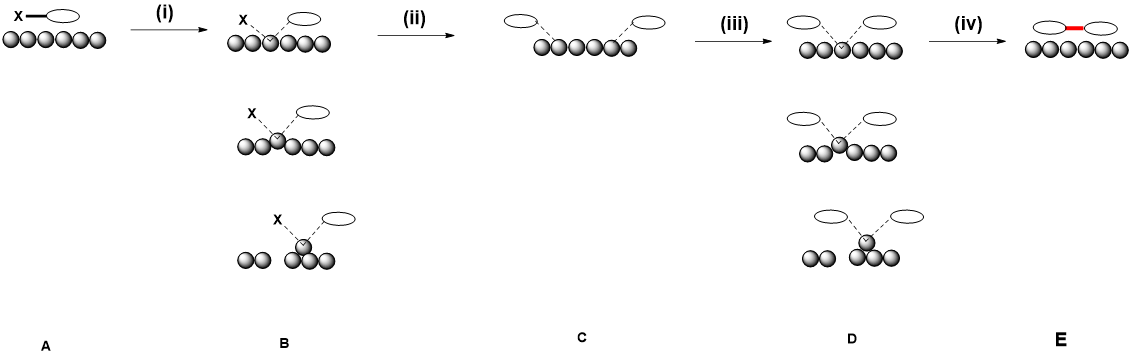
\includegraphics[width=0.9\textwidth]{Fig/mechanism.png}
\caption{Elementary steps of a surface Ullmann Coupling reaction mechanism}
\label{fig_mecha}
\end{figure*}
%(ZZ: I suggest we change the mechanism figure here, maybe emphasize the possible intermediates in the text?)
%RZK1219: Agreed. This needs to be discussed in detail, but this is not yet a high-priority task.

%RZZK: Summarize the focus of the following review: halogens as the leaving group, Cu,Ag,Au metals, narrower focus on monohalogenated benzene. Emphasize that we review C--C bond formation, not carbon-heteroatom bond formation.

%%\begin{enumerate}[align=left, itemindent=2em, label=(\roman*)]
    %%\item Dehalogenation of Precursors [The fundamental step is the %%disassociate of halogens, the cleavage of C-X bonds (X = halogens) is %%usually activated by thermal, electron-induced and photon-simulated. %%The energy will vary from 0.05 ~ 0.80 eV with different X on different %%coinage surfaces.]
    %%\item Diffusion of single Dehalogenlated 'Radicals' [The removal of %%halogens from precursors results in unsaturated carbons (radicals), %%which interact with metal atoms to form C-Metal radical (C = %%dehalogenated precursor and Metal = Au, Ag or Cu). C-Metal radical %%will diffuse on metal surface and the metal atom interacting with the %%radical will shift.]
    %%\item The Formation of Organometallic Intermediates C-Metal-C from Two %%Single Radicals [Diffusion brings two single radical close to each %%other, and then these two species would form a dimerized %%organometallic intermediate before the appearance of coupling product]
    %%\item The Formation of Carbon-Carbon Bond []
    %%\item Diffusion of Coupling Product []
%%\end{enumerate}  

\subsubsection{Dehalogenation}

%RZK1217: Have we ever discussed carbon--heteroatom bond formation on the SURFACE in this review? If not, I will make a comment in the text about this. 
The first fundamental step of surface Ullmann coupling is the dissociative dehalogenation of organic precursors adsorbed on the surface. In this step, the carbon-halogen bonds of the precursor are broken whereas the carbon-metal and halogen-metal bonds are formed. The thermodynamics and kinetics of the process are primarily determined by the relative strength of the broken and formed bonds, shown below. 

\rule{\columnwidth}{0.4pt}

The following trends in the bond strength have been derived from model molecular systems.
%
\begin{eqnarray}
\begin{split}
\text{C--Cl} > \text{C--Br} > \text{C--I} \\ 
\text{Cu--C} > \text{Au--C} > \text{Ag--C} \\
\text{Cu--Cl} > \text{Cu--Br} > \text{Cu--I}\\
\text{Ag--Cl} \approx \text{Ag--Br} > \text{Ag--I} \\
\text{Au--Cl} > \text{Au--I} > \text{Au--Br}
\end{split}
\end{eqnarray}
%
The bond dissociation energy of diatomic and CX$_4$ molecules have been used in the cases of the metal-halogen bonds~\cite{ullmann_62} and carbon-halogen bonds~\cite{ullmann_63}, respectively. The relative strength of metal-carbon bond strength has been estimated using the metal-carbon bond distances in M-(CH$_3$)$_2$ molecules~\cite{ullmann_61}.
%RZK1219: references above are missing from the bib file.

For the surface Ullmann coupling reaction, the metal-halogen bond strength can be arranged in the following series.
%RZZK: What is the origin of this series? It is completely unclear from your description. Experiments or theory? Temperature measurements? You do not cite where this series came from. This is the last three rows above combined.
%
\begin{gather*}
\text{Cu--Cl} > \text{Cu--Br} > \text{Au--Cl} \approx \text{Au--I} \approx \text{Ag--Br} \approx \\
 \approx \text{Ag--Cl} > \text{Ag--I} > \text{Au--Br} > \text{Cu--I}
\end{gather*}
%RZK1219: Is the series above sufficient to predict differences in the thermodynamics and kinatics of the first step? How? Metal-halogen is just one of the factors mentions above.
%RZK1219: What of the two factors influence this step more: the nature of the halogen or the nature of the metal? It is possible to do a whole study on the predicting the energetics of this step based on bond energies. This can be done in the results and discussion, if necessary.

This data illuminates the strong influence of surfaces on the first step of the reaction. % which has been proven in experiment of bromobenzene and iodobenzene. 
For instance, the dissociaton of iodobenzene occurs at approximately 175~K on Cu(111)~\cite{sur_sci01}, 200~K on Ag(111)~\cite{sur_sci02} and 250~K on Au (111)~\cite{sur_sci03}. 
%RZK1221: It is unclear what "occurs" refers to. Dissociation happens even at very low temperture but to a lesser degree. 
%RZK1221: The strengths of bonds actually predict the opposite order in temperatures.
The same trend has been observed for bromobenzene with a higher temperature on all surfaces.
%RZK1221: For Br-Metal, the trend in strength is reversed. How this can be explained?

DFT calculations have estimated the activation barrier for the exothermic dehalogenation of bromobenzene and iodobenzene on (111) metal surfaces to be 0.4--1.0~eV~\cite{jacs2013}. As shown in Fig.~\ref{fig:dehalo}, the activation barrier and reaction energy decrease in the order Au $>$ Ag $>$ Cu and are 0.1--0.5 eV lower for iodobenzene than bromobenzene. The latter is due to the dissociation energy of a C--I bond being $\sim$0.65~eV lower than that of a C--Br bond~\cite{Arpc1982}.

} %lock

%%%%%%%%%% old text %%%%%%%%%%%%%%%
%RZK1219.
\rule{\columnwidth}{0.4pt}

RZK: The following text is what you submitted for this subsection. Compare it to my text above. Go to the \LaTeX\ source and perform diff line by line. The most important comments are in the email.

\rule{\columnwidth}{0.4pt}

Bond strength (X = Halogen):
%RZZK: I did not check the actual strength for these bonds, please check the trends (%ZZ: checked and literature attached)
%
\begin{eqnarray}
\begin{split}
\text{C -- Cl} > \text{C -- Br} > \text{C -- I} \\ 
\text{Cu -- C} > \text{Au -- C} > \text{Ag -- C} \\
\text{Cu -- Cl} > \text{Cu -- Br} > \text{Cu -- I}\\
\text{Ag -- Cl} \approx \text{Ag -- Br} > \text{Ag -- I} \\
\text{Au -- Cl} > \text{Au -- I} > \text{Au -- Br}
\end{split}
\end{eqnarray}
(M-X bond strength is compared according to bond dissociation energy of diatomics~\cite{ullmann_62}, C-X bond strength according to the bond dissociation energy in CX$_4$ molecule~\cite{ullmann_63}, M-C bond strength according to the metal-carbon bond distance in M-(CH$_3$)$_2$~\cite{ullmann_61}).
For surface Ullmann coupling reaction, M-X bond strength can be compared together to present an overall relationship.

\begin{gather*}
\text{Cu -- Cl} > \text{Cu -- Br} > \text{Au -- Cl} \approx \text{Au -- I} \approx \text{Ag -- Br}\\
 \approx \text{Ag -- Cl} > \text{Ag -- I} > \text{Au -- Br} > \text{Cu -- I}
\end{gather*}
%
%RZZK: Experimental trends in the halogen series. Compare observables (for example, dissociation temperature) for X=I,Br,Cl and the same metal (say, Cu). (%ZZ: added)
%RZZK: What of the two factors influence this step more: the nature of the halogen or the nature of the metal? Is it possible to arrange the nine M--X cases in term of bond strength? It is possible to do a whole study on the predicting the energetics of this step based on bond energies. This can be done in the results and discussion, if necessary. (%ZZ: added)
This data also indicate the distinct influence of surfaces, which has been proven in experiment of bromobenzene and iodobenzene. For instance, the dissociaton of iodobenzene occurs at approximately 175~K on Cu(111)~\cite{sur_sci01}, 200~K on Ag(111)~\cite{sur_sci02} and 250~K on Au (111)~\cite{sur_sci03}. The same trend has been demonstrated by bromobenzene with a higher T on all surfaces.

Björk \textit{et al.} ~\cite{jacs2013} proposed an activation barrier of 0.4-1.0 eV for exothermic dehalogenation by DFT simulations. In specific, bromobenzene and iodobenzene on Au(111), Ag(111) and Cu(111) surface displayed different reactivity, i.e., the activation barrier and reaction energy both decrease in the order Au $>$ Ag $>$ Cu, and for all surfaces studied, iodine substituent are 0.1-0.5 eV lower than bromine ones in dehalogenation As shown in Fig.~\ref{fig:dehalo}. The trend is plausible due to the Bond-dissociation energy (BDE) of C-I is ~0.65 eV lower than C-Br\cite{Arpc1982}.

\rule{\columnwidth}{0.4pt}
%%%%%%%%%% end old text %%%%%%%%%%%%%%%


\begin{figure}[tbh]
\centering
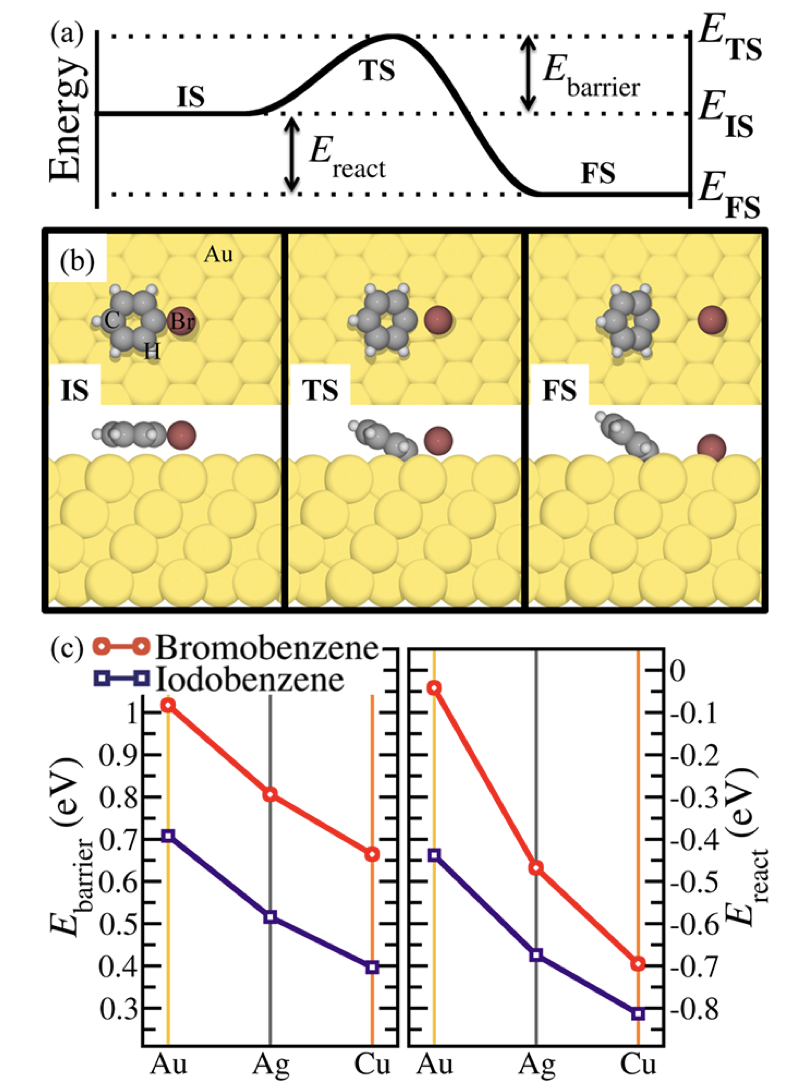
\includegraphics[width=0.75\columnwidth]{Fig/dehalogentaion.png}
\caption{Figure 1. (a) Definitions of the energy barrier ($E_{barrier}$) and reaction energy ($E_{react}$) for dehalogenation reactions. (b) The dissociation of bromobenzene on Au(111), depicting top and side views of the initial state (IS), transition state (TS), and final state (FS) of the reaction. (c) $E_{barrier}$ (left) and $E_{react}$ (right) for the dissociation of bromobenzene and iodobenzene on the (111) facets of Au, Ag, and Cu.} 
%RZK: Detailed description of the figure. Take a look at the original publication. Reprinted from~\cite{RZK} with permission of American Chemical Society or PUBLISHER. See the LaTeX comment below.
%%RZK: If you take a figure from a publication it is very important to cite the work and obtain publisher's permission. We need to make sure that all our borrowed figures satisfy copyright permissions. For example, see: https://www.stm-assoc.org/2016_01_05_Guidelines_for_Quotation_From_Journal_Articles.pdf (%ZZ: need to discuss)
\label{fig:dehalo}
\end{figure}

{\color{blue}
%RZK1217: Have we ever discussed carbon--heteroatom bond formation on the SURFACE in this review? If not, I will make a comment in the text about this. (%ZZ1225: no, we did not discuss on this)
The first fundamental step of surface Ullmann coupling is the dissociative dehalogenation of organic precursors adsorbed on the surface. In this step, the carbon-halogen bonds of the precursor are broken whereas the carbon--metal and halogen--metal bonds are formed. The thermodynamics and kinetics of the process are primarily determined by the relative strength of the broken and formed bonds, shown below. 


The following trends in the bond strength have been derived from model molecular systems.
%
\begin{eqnarray}
\begin{split}
\text{C--Cl} > \text{C--Br} > \text{C--I} \\ 
\text{Cu--C} > \text{Au--C} > \text{Ag--C} \\
\text{Cu--Cl} > \text{Cu--Br} > \text{Cu--I}\\
\text{Ag--Cl} \approx \text{Ag--Br} > \text{Ag--I} \\
\text{Au--Cl} > \text{Au--I} > \text{Au--Br}
\end{split}
\end{eqnarray}
%
The bond dissociation energy of diatomic and CX$_4$ molecules have been used in the cases of the metal-halogen bonds~\cite{ullmann_62} and carbon-halogen bonds~\cite{ullmann_63}, respectively. The relative strength of metal-carbon bond strength has been estimated using the metal-carbon bond distances in M--(CH$_3$)$_2$ molecules~\cite{ullmann_61}.
%RZK1219: references above are missing from the bib file. (%ZZ: solved)

If the strength of all kinds of metal-halogen bonds shown above are compared in conjunction, the order can be arranged in the following series.
%RZZK: What is the origin of this series? It is completely unclear from your description. Experiments or theory? Temperature measurements? You do not cite where this series came from. This is the last three rows above combined.
%
\begin{gather*}
\text{Cu--Cl} > \text{Cu--Br} > \text{Au--Cl} \approx \text{Au--I} \approx \text{Ag--Br} \approx \\
 \approx \text{Ag--Cl} > \text{Ag--I} > \text{Au--Br} > \text{Cu--I}
\end{gather*}
%RZK1219: Is the series above sufficient to predict differences in the thermodynamics and kinetics of the first step? How? Metal-halogen is just one of the factors mentions above.
%RZK1219: What of the two factors influence this step more: the nature of the halogen or the nature of the metal? It is possible to do a whole study on the predicting the energetics of this step based on bond energies. This can be done in the results and discussion, if necessary.

This data illuminates the strong influence of surfaces on the first step of the reaction. % which has been proven in experiment of bromobenzene and iodobenzene. 
For instance, the dissociaton of iodobenzene occurs at $\sim$\SI{175}{\kelvin} on Cu(111)~\cite{sur_sci01}, $\sim$\SI{200}{\kelvin} on Ag(111)~\cite{sur_sci02} and $\sim$\SI{250}{\kelvin} on Au (111)~\cite{sur_sci03}. 
%RZK1221: It is unclear what "occurs" refers to. Dissociation happens even at very low temperature but to a lesser degree. 
%RZK1221: The strengths of bonds actually predict the opposite order in temperatures.
The same trend has been observed for bromobenzene with a higher temperature on all surfaces.
%RZK1221: For Br-Metal, the trend in strength is reversed. How this can be explained?

DFT calculations have also estimated the activation barrier for the exothermic dehalogenation of bromobenzene and iodobenzene on (111) metal surfaces to be \SIrange{0.4}{1.0}{\electronvolt}~\cite{jacs2013}. As shown in Fig.~\ref{fig:dehalo}, the activation barrier and reaction energy decrease in the order Au $>$ Ag $>$ Cu and are \SIrange{0.1}{0.5}{\electronvolt} lower for iodobenzene than bromobenzene. The latter is due to the dissociation energy of a C--I bond being $\sim$\SI{0.65}{\electronvolt} lower than that of a C--Br bond~\cite{Arpc1982}.

}


\subsubsection{Diffusion}

{\lock

The dehalogenation step produces organometallic intermediates with carbon atoms covalently bonded directly to surface metal atoms. 
%RZZK: These species are often referred to as radicals even though it remains unclear whether their possess unpaired electrons.
The diffusion of these species, which has been observed experimentally and studied computationally, plays a decisive role in the further coupling process. 
The ease diffusion increases the probability that two molecules move closer to each other resulting in the creation of the bond between them.

}


An STM imaging has revealed that dehalogenated phenyl groups diffuse on Cu(111) at [temperatures as low as] 77~K~\cite{langm01}. The energy barrier of the diffusion has been calculated to be approximately 0.09~eV. %RZK1223: citation is missing for calculations

%RZK1221. You still use Figure instead of Fig. in your text. Search the entire text for figure and relace where appropriate.
%RZK1221: There are no references to flipping/sliding mechanisms.
Phenyl has been proposed to diffuse either by sliding or flipping. In the sliding mechanism, phenyl groups keep their surface orientation in the initial and final states and the energy barriers of diffusion on different metal surface follow the order Cu(111) $>$ Ag(111) $>$ Au(111). 
%RZK1220: It appears that you discuss 3 things: overturn, sliding, flipping. How overturning is different from flipping? What is sliding? Better structure, sequence of thoughts, is needed.
%RZK1221: I have stated this before and I have to emphasize this one more time that you should use PRESENT PERFECT tense, not PAST SIMPLE when you report previous findings. Do not use PAST tense to report hings that are universally TRUE, use PRESENT SIMPLE. For example, "The energy barriers follow", not ""The energy barriers followed"
For the flipping mechanism, it has been shown that phenyl groups, which are tilted at $\sim 36^\circ$ with respect to the surface~\cite{pccp2010, jacs2013}, overturn during the diffusion and then bind to a nearby metal atom as shown in Fig.~\ref{fig:4}.
For the this type of diffusion, the height of diffusion barriers decreases Au(111) $>$ Cu(111) $>$ Ag(111). 
%RZK1221: why different order? Is it something that can be understood from simple bonding arguments?
Since the flipping mechanism has a lower energy barrier, it has been proposed as the most plausible mechanism for the diffusion of phenyl groups on metal surfaces. 
%RZK1221: Since you compare barriers, is it important to write the barrier heights for the sliding/flipping mechaniss?
%RZK1221: I disagree that the mechanism with the lowest barrier of diffusion is the dominant mechanism. If both barriers are low then both mechanism will contribute.

\begin{figure}[htb]
\centering
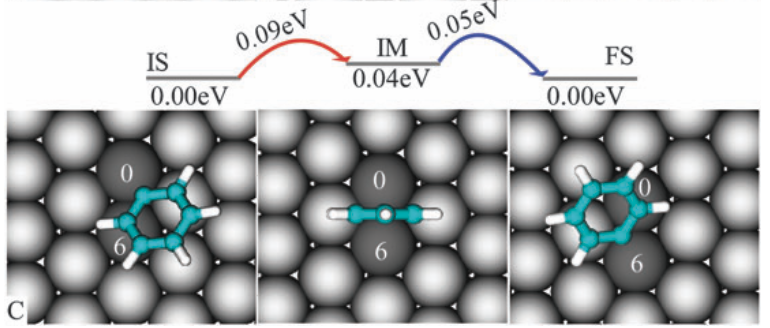
\includegraphics[width=0.75\columnwidth]{Fig/overturn.png}
\caption{Diffusion of phenyl group on Cu(111): phenyl group migrates from Cu0 to the neighboring metal atoms} %RZK: better caption, copyright. (%ZZ: added)
\label{fig:4}
\end{figure}

%RZZK: The following needs to be stated in the end. The diffusion energy barrier and the tilt angle between single radical and substrate will change with the size increasing of reactant molecules.

%RZK1221: Do not mention the year of publication if you do not describe the history of research. Do not mention authors unless this is important.
Besides the organometallic intermediates, halogen atoms chemisorbed on the surface undergo the diffusion process. 
The binding energy of halogens and their diffusion barriers have been investigated using DFT calculations~\cite{jacs2013}.
%RZK1221: Do not capitalize names of elements.
%RZK1221: How do we know that they display high mobility? Is it observed or is it inferred from calculations?
Bromine and iodine atoms [are expected to?] display high mobility at experimental temperature due to small energy barriers in the range of 50-100 mv on Cu(111), Ag(111), and Au(111). The barrier for the halogen diffusion is the highest on Au(111) and lowest on Cu(111). 
%RZK1221: mv is not a unit of energy, check, convert to eV and report properly. Do we know the barriers for all three surfaces? If yes, report them here.

{\color{blue}
The dehalogenation step produces organometallic intermediates with carbon atoms covalently bonded directly to surface metal atoms. 
%RZZK: These species are often referred to as radicals even though it remains unclear whether their possess unpaired electrons.
The diffusion of these intermediates, which has been observed experimentally and studied computationally, plays a decisive role in the further coupling process. Species on surface Prone to diffuse will enable them move closer to each other then results in the construction of new bonds. 


%It has been observed that dehalogenated phenyl groups diffuse on Cu(111) at temperatures as low as \SI{77}{\kelvin}~\cite{langm01} in STM. The energy barrier of the diffusion has also been calculated to be $\sim$\SI{0.09}{\electronvolt}~\cite{pccp2010}.
%RZK1223: citation is missing for calculations{%ZZ: solved}

%RZK1221. You still use Figure instead of Fig. in your text. Search the entire text for figure and replace where appropriate.
%RZK1221: There are no references to flipping/sliding mechanisms.
Among all the delogenated precursors, phenyl groups are studied the most widely. Phenyl has been proposed to diffuse either by sliding or flipping fashions~\cite{jacs2013}. In the sliding mechanism, phenyl groups remain their orientation to the surface in the initial, transition and final states, the energy barriers of diffusion on different metal surface decrease in the order Cu(111) $>$ Ag(111) $>$ Au(111). It has been observed that dehalogenated phenyl groups can diffuse on Cu(111) at temperatures as low as \SI{77}{\kelvin}~\cite{langm01} using STM.
%RZK1220: It appears that you discuss 3 things: overturn, sliding, flipping. How overturning is different from flipping? What is sliding? Better structure, sequence of thoughts, is needed.
%RZK1221: I have stated this before and I have to emphasize this one more time that you should use PRESENT PERFECT tense, not PAST SIMPLE when you report previous findings. Do not use PAST tense to report hings that are universally TRUE, use PRESENT SIMPLE. For example, "The energy barriers follow", not ""The energy barriers followed"
For the flipping mechanism, it has been shown that phenyl groups, which are tilted at $\sim$\SI{36}{\degree} with respect to the surface~\cite{pccp2010, jacs2013} at the beginning, will overturn during the diffusion and then bind to an adjacent metal atom as shown in Fig.~\ref{fig:4}.
For this type of diffusion, the magnitude of diffusion barriers decreases in the order Au(111) $>$ Cu(111) $>$ Ag(111). 
%RZK1221: why different order? Is it something that can be understood from simple bonding arguments? (%ZZ: I did not find any comments on original paper, should we add our own explanation?)
For simple phenyl groups, the flipping diffusion is concerned with a smaller energy barrier compared to the sliding diffusion. On Cu(111), Ag(111) and Au(111) surface, the barrier of flipping was reported to be \SI{0.4}{\electronvolt}, \SI{0.25}{\electronvolt} and \SI{0.05}{\electronvolt} lower than sliding fashion respectively~\cite{jacs2013}. 
In experiments, the diffusion of phenyl groups always occurs at a very low temperature~\cite{langm01}. Since the energy barriers of sliding and flipping mechanism are realistically low, we can consider that both fashions will take place in nature. However, the flipping mechanism may not be favorable for precursor in larger size, the stronger physisorption between the larger molecules and surface will drive the molecule plane more parallel to the surface, such as cyclohexa-m-phenylene~\cite{ullmann_65}.
%RZK1221: Since you compare barriers, is it important to write the barrier heights for the sliding/flipping mechaniss?
%RZK1221: I disagree that the mechanism with the lowest barrier of diffusion is the dominant mechanism. If both barriers are low then both mechanism will contribute.

%RZZK: The following needs to be stated in the end. The diffusion energy barrier and the tilt angle between single radical and substrate will change with the size increasing of reactant molecules.

%RZK1221: Do not mention the year of publication if you do not describe the history of research. Do not mention authors unless this is important.
In addition to organometallic intermediates, halogen atoms dissociated from the precursors will be chemisorbed by the surface and also undergo the diffusion process. 
There are few experiment works related to the diffusion of halogen atoms on metal surface, but it is much better investigated theoretically using DFT calculations~\cite{ullmann_66}.
%RZK1221: Do not capitalize names of elements.
%RZK1221: How do we know that they display high mobility? Is it observed or is it inferred from calculations? (%ZZ: few work)
Atomic bromine is reported to have a diffusion energy barrier of \SI{0.09}{\electronvolt}, \SI{0.07}{\electronvolt} and \SI{0.06}{\electronvolt} on Au(111), Ag(111) and Cu(111) respectively. Atomic Iodine have a barrier of \SI{0.11}{\electronvolt}, \SI{0.06}{\electronvolt} and \SI{0.06}{\electronvolt} on Au(111), Ag(111) and Cu(111) respectively. And atomic chlorine have a barrier of \SI{0.02}{\electronvolt} and \SI{0.08}{\electronvolt} on Au(111) and Cu(111) respectively. The diffusion barrier for atomic halogens are very low, which is expected to lead to a high mobility of halogen species on metal surface.

%Bromine and iodine atoms [are expected to?] display high mobility at experimental temperature due to small energy barriers in the range of 50-100 mv on Cu(111), Ag(111), and Au(111). The barrier for the halogen diffusion is the highest on Au(111) and lowest on Cu(111). 
%RZK1221: mv is not a unit of energy, check, convert to eV and report properly. Do we know the barriers for all three surfaces? If yes, report them here.
Since all species produced in surface Ullamnn coupling are mobile on metal surface, further C--C bond formation and covalent assembled structure will be highly determined by the diffusion process.


}

\subsubsection{Formation of carbon--metal--carbon(C--M--C) structure intermediates} \label{sec:dimerized}
%RZZK: Dimerization??? (%ZZ two organometallic intermediates bond together)

{\lock

Dimerized organometallic intermediates will form when two organic fragments diffuse close to each other and become bound to the same metal atom, without yet creating a direct covalent bond. Since the distance between two carbon atoms in such carbon-metal-carbon bridges is significantly larger than in a covalent bond, their existence has been confirmed in multiple STM~\cite{jacs2011}, tunneling RZK~\cite{RZK} and other experimental studies, typically accompanied by DFT calculations~\cite{RZK}.

}

{\color{blue}
C--M--C structure intermediates will form when two single organometallic fragments diffuse close to each other and bound to the same metal atom, without yet creating a direct C--C covalent bond. Since the distance between two carbon atoms in such C--M--C bridge structure is significantly larger than in a covalent bond, their existence has been confirmed in multiple STM~\cite{jacs2011}, tunneling RZK~\cite{RZK} and other experimental studies, typically accompanied by DFT calculations~\cite{ullmann_67}.
%ZZ1228: tunneling?

For simple phenyl groups, STM images prove that the intermediate structure consisting of two phenyl groups bound to the same Cu atom will form on Cu(111) surface at \SI{160}{\kelvin}, as shown in Fig.~\ref{fig:organ}. The measured length of these intermediate structures agree well with the theoretical length of two Cu--C bonds and two phenyl diameters~\cite{ullmann_67}. And the dissociated halogen atoms are distributed closely around these intermediate structures. The activation energy of forming such C--M--C bridge structure from two single organometallic intermediates is reported to be \SI{0.38}{\electronvolt}\cite{pccp2010}. 

More kinds of precursors have been investigated in this stage other than phenyl groups. Dibromoterphenyl on Cu(111) and Ag(111) surface was proven to form C--Cu--C bridges and C--Ag--C bridges both at \SI{300}{\kelvin}, since length of the intermediate characterized by STM is consistent with DFT calculated length of terphenyl--Cu/terphenyl--Ag groups. Projected density of states also indicate the existence of C--Cu--C/C--Ag--C bridge structures~\cite{jacs2011, PCCP2012}. These two bridge structures were both obtained at \SI{300}{\kelvin}, which revealed that the barrier for two terphenyl groups
coordinated with Ag atom and Cu atom are close. 

Compared to the dehalogenation, this step requires generally \SIrange{150}{200}{\kelvin} higher temperature condition (still near room temperature in most cases). On Cu and Ag surface, the C--Cu--C and C--Ag--C bridge structures are always observed, but on Au surface C--Au--C are occasionally reported. This is explained by a relatively low eneryg barrier of conversion from this state to final covalent bond formation on Au surface, resulting in a very short life time of C--Au--C existence~\cite{ullmann_33}.



}
%RZK1221: Is there any specific reason you want to provide such a detailed description here. You do not describe research in such a level of detail for other steps. So, unless there is a good reason to provide details, this must be reduced just to key facts about this step. What facts do you want to emphasize? (%ZZ: I simplify it)
%Temperature required for this step to occur is higher that temperature for dehalogenation. How general is this trend?
%Au is different from Cu and Ag. Again, how general is the trend?

In 2011, Wang \textit{et al.}~\cite{jacs2011} studied the organometallic intermediate of surface Ullmann coupling from dibromoterphenyl to polyphenylene using STM and DFT calculations [on copper?]. 
When the temperature went to 300~K, both Br atoms were dissociated from the phenyl group. However, the length of linear periodic structure formed in reaction (characterized by STM) was 4.8~\AA\ longer than the length of DFT calculated terphenyl group (ph)$_{3}$, which indicated the possibility that copper atoms were inserted and served as linkage parts inside terphenyl groups. Besides, performed tunneling spectra (dI/dV) of one periodic unit of the experimental formed structure and the calculated projected density of states (PDOS) of (ph)$_{3}$/Cu atom both showed the same value at ~2.7 eV, which further proved the existence of C-Cu-C bridges in organometallic intermediate structures, all the evidences are shown in Fig.~\ref{fig:organ}. Similar methods have been used by Chung \textit{et al.}~\cite{PCCP2012} with the same molecules on Ag(111). C-Ag-C bridges were observed and demonstrated in the organometallic intermediates.

The C-Ag-C and C-Cu-C structures were both obtained at 300 K, which revealed that the barrier for two terphenyl
coordinated with Ag and Cu are close. Compared to the dehalogenation, this step requires a higher temperature condition (still near room temperature). On Cu and Ag surface, the dimerized organometallic intermediates are always observed, but on Au surface are occasionally reported. This is explained by a relatively low barrier conversion from this state to covalent bond formation on Au surface, resulting in a very short life time of C-Au-C existence~\cite{ullmann_33}.

%RZK1221: Since the focus here is on mono-substituted benzene, is there anything known about this step for Ph-Hal? (%ZZ: added)

%RZK1221: It is not worth diplaying this figure. It is not ver informative. If we are to place a figure here, it is better to use one that clearly shows the structure of the dimerized intermediate, perhaps from simulations.
\begin{figure}[ht]
\centering
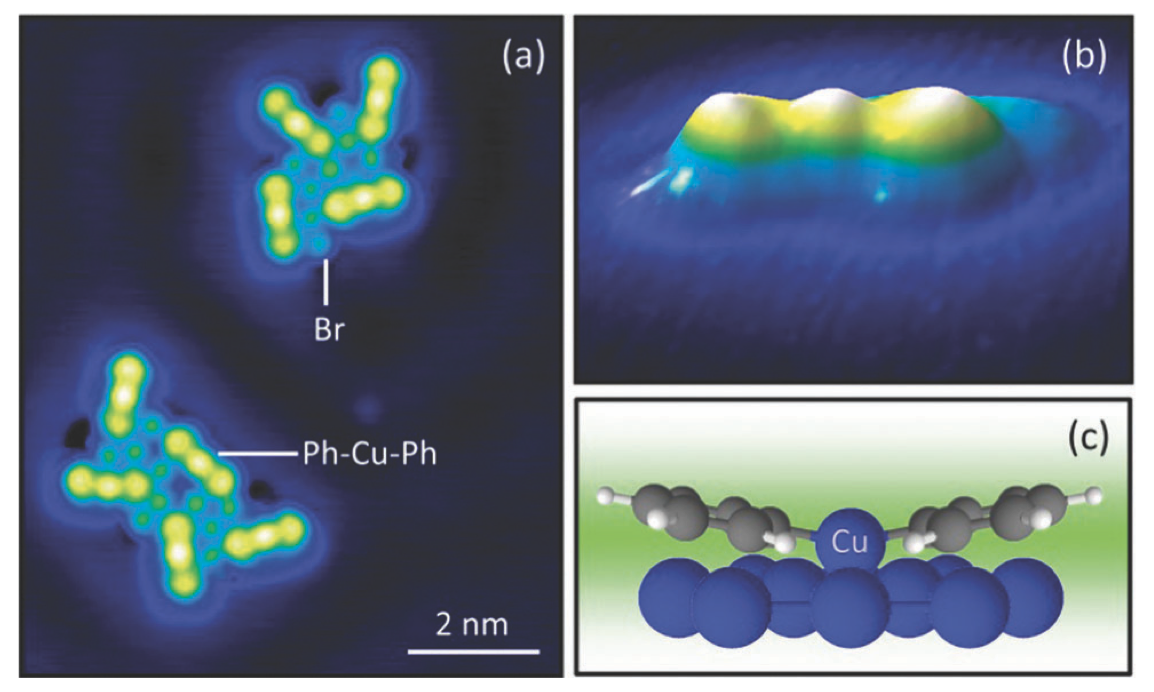
\includegraphics[width=0.75\columnwidth]{Fig/phenylorgano.png}
\caption{STM images and model showing the assembly and high-resolution details of the organometallic intermediate. All imaging at \SI{5}{\kelvin}. Structure are formed at \SI{160}{\kelvin} (a) Clusters of the organometallic intermediates and Br atoms. Scale bar = \SI{2}{\nm}. (b) 3D rendering of a single phenyl–Cu–phenyl intermediate, illustrating the shape of the species. (c) Model showing the proposed bonding configuration of the phenyl species to the Cu atom.}
\label{fig:organ}
\end{figure}



\subsubsection{Formation of the C--C bond}

{\color{blue}
After further annealing, the metal atoms will be released from the C--M--C structure intermediates, spontaneously a covalent bond will be irreversibly constructed between these two carbon atoms. The formation of C--C bond in this stage has been widely explored in experiment and theoretically as well.

Biphenyl products are reported to form from two phenyl groups at \SI{350}{\kelvin} on Cu(111) surface in experiment~\cite{ullmann_68, ullmann_69}. DFT calculation also demonstrates the energy change and energy barrier for this step~\cite{jacs2013}. As shown in Fig.~\ref{fig:coupling}, the energy change of forming biphenyl on difference metal surface decreases in the order Ag $>$ Au $>$ Cu, and the energy barrier decreases in the order Ag $>$ Cu $>$ Au. The formation the C--C bond for two phenyl groups appears to be highly exothermic for all surfaces.


\begin{figure}[ht]
\centering
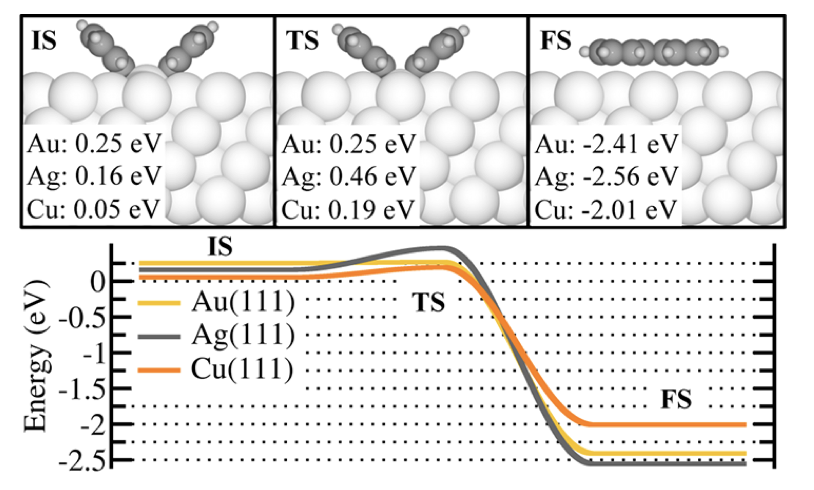
\includegraphics[width=0.75\columnwidth]{Fig/couplingenergy.png}
\caption{Energy diagram for the coupling reaction of two phenyls into biphenyl on the of Au(111), Ag(111), and Cu(111). In the top panel, the reaction is depicted for Ag(111), with the energy indicated for each of the states along the path for the respective surface. The energies are given with respect to the most stable adsorption configuration of an isolated phenyl on the respective surface.}
\label{fig:coupling}
\end{figure}

More types of molecules were also reported, such as the dimerization and trimerization of 1,4-dibromobenzene on Cu(100) surface. DFT calculations shows that the activation energy of formation of C--C bond in dimer and trimer are \SI{0.7}{\electronvolt} and \SI{0.2}{\electronvolt}, respectively~\cite{jacs2016}. This value is consistent with the experiment temperature condition for dimerization of 1,4-dibromobenzene, typically \SI{500}{\kelvin} is required for this molecule to construct a C--C bond on Cu(100).
%RZK1221: Higher than what?
%RZK1212: Is it important what surface? 111 or other or it does not matter.

In general, this final step requires the highest annealing temperature in surface Ullmann coupling process. Like for dihalobenzene (halo = Cl, Br or I) precursor on Cu(110), the formation of C--C bond requires a temperature ranging from \SIrange{410}{450}{\kelvin}, which is higher than the temperature needed to process the dehalogenation in the range from \SIrange{170}{370}{\kelvin}~\cite{ullmann_44}. On other type of Cu surface, as well on Ag and on Au surface, a higher annealing temperature for C--C coupling has also been reported than dehalogenation steps~\cite{ Naturenano2007, ullmann_70, ullmann_71}. 

%This indicates that the energy barrier of the formation of C--C bond step on three metal surfaces should decrease in the order Au $>$ Cu $>$ Ag.
%%%%%%%%%%%%%%%%%%%%%%%%%%%%%%%%%%%%%%%%%%%%%%%%%%%%%%%%%%%%%%%%%%%%%%%%%%
%RZK1221: Is it your speculation? If yes, it should be in Results and Discussion. If not, a reference should be given.(%ZZ: will discuss in result part)
%And since there were limited reports on the formation of C--Au--C intermediates, it could be safely speculated that a high energy barrier exists in the formation of C-Au-C dimerized organometallic intermediates and a low barrier exists in the covalent bond formation.
%%%%%%%%%%%%%%%%%%%%%%%%%%%%%%%%%%%%%%%%%%%%%%%%%%%%%%%%%%%%%%%%%%%%%%%%%%

%\begin{figure}[ht]
%\centering
%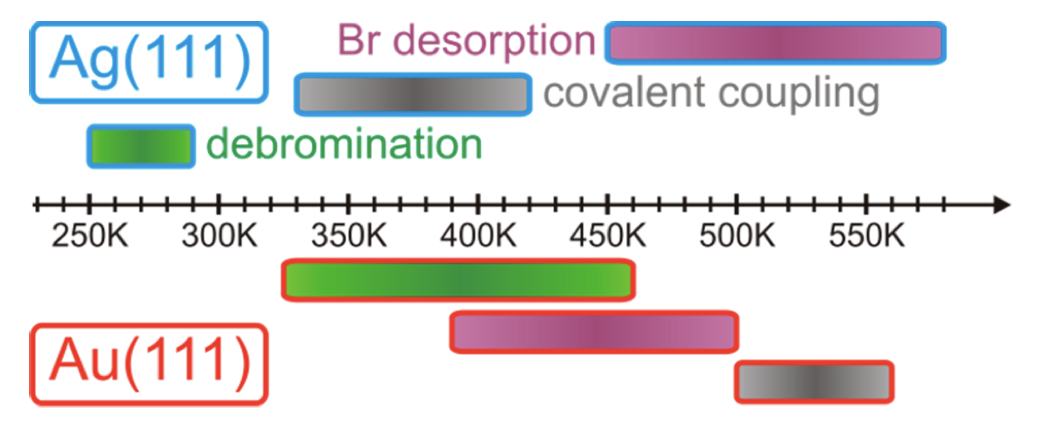
\includegraphics[width=0.75\columnwidth]{Fig/steptemp.png}
%\caption{Overview and Comparison of the Temperature Ranges for Debromination (Green), Covalent Coupling (Gray), and Thermal Desorption of Bromine (Violet) on Ag(111) (Top) versus Au(111) (Bottom) As Deduced from Both Br 3d and C 1s TP-XPS Data}
%\label{fig:temp}
%\end{figure}



With the formation of C--C bond, a surface Ullmann coupling would be completed between two monomers, resulting in a dimer. If there are more than one functional groups on a monomer, this dimer could further diffuse and couple to obtain a trimer~\cite{jacs2016}, and oligomers~\cite{ullmann_53, ullmann_56} or polymers~\cite{ullmann_43, ullmann_54, ullmann_55}.

}
After further annealing, the metal atoms are released from the dimerized organometallic intermediates, spontaneously a covalent bond will be irreversibly constructed between two carbon atoms. The formation of C--C bond in this state has also been widely explored in experiment and theoretically as well.

%RZK1221: Results for phenyl-halogens must be described here first.

It has been reported~\textit{et al.}~\cite{jacs2016} that the dimerization and trimerization of 1,4-dibromobenzene on Cu(100) in UHV condition and related simulations with DFT methods. DFT results show that the dimerized organometallic intermediate is a  stable phase in the potential energy surface. A 0.7 eV of activation energy was required from the dimerized organometallic intermediate to the coupling dimer. And a 0.2 eV of activation was needed for the coupling dimer to produce the trimer product, the data could be reviewed in Fig.~\ref{fig:dimer}. 
%RZK1221: Again, you give to many irrelevant details for a short review. If the 2013 work gives the same results, combine it with the previous sentence.
These data are consistent with Di Giovannantonio's another experiment work~\cite{acsnano2013} in 2013. Same precursor 1,4-dibromobenzene was deposited on Cu(100) surface and the surface Ullmann coupling process was pictured in STM image. It was reported that organometallic intermediates were formed at room temperature, nevertheless the final formation of C--C bond needed an annealing temperature up to 500 K.

%\begin{figure*}[ht]
%\centering
%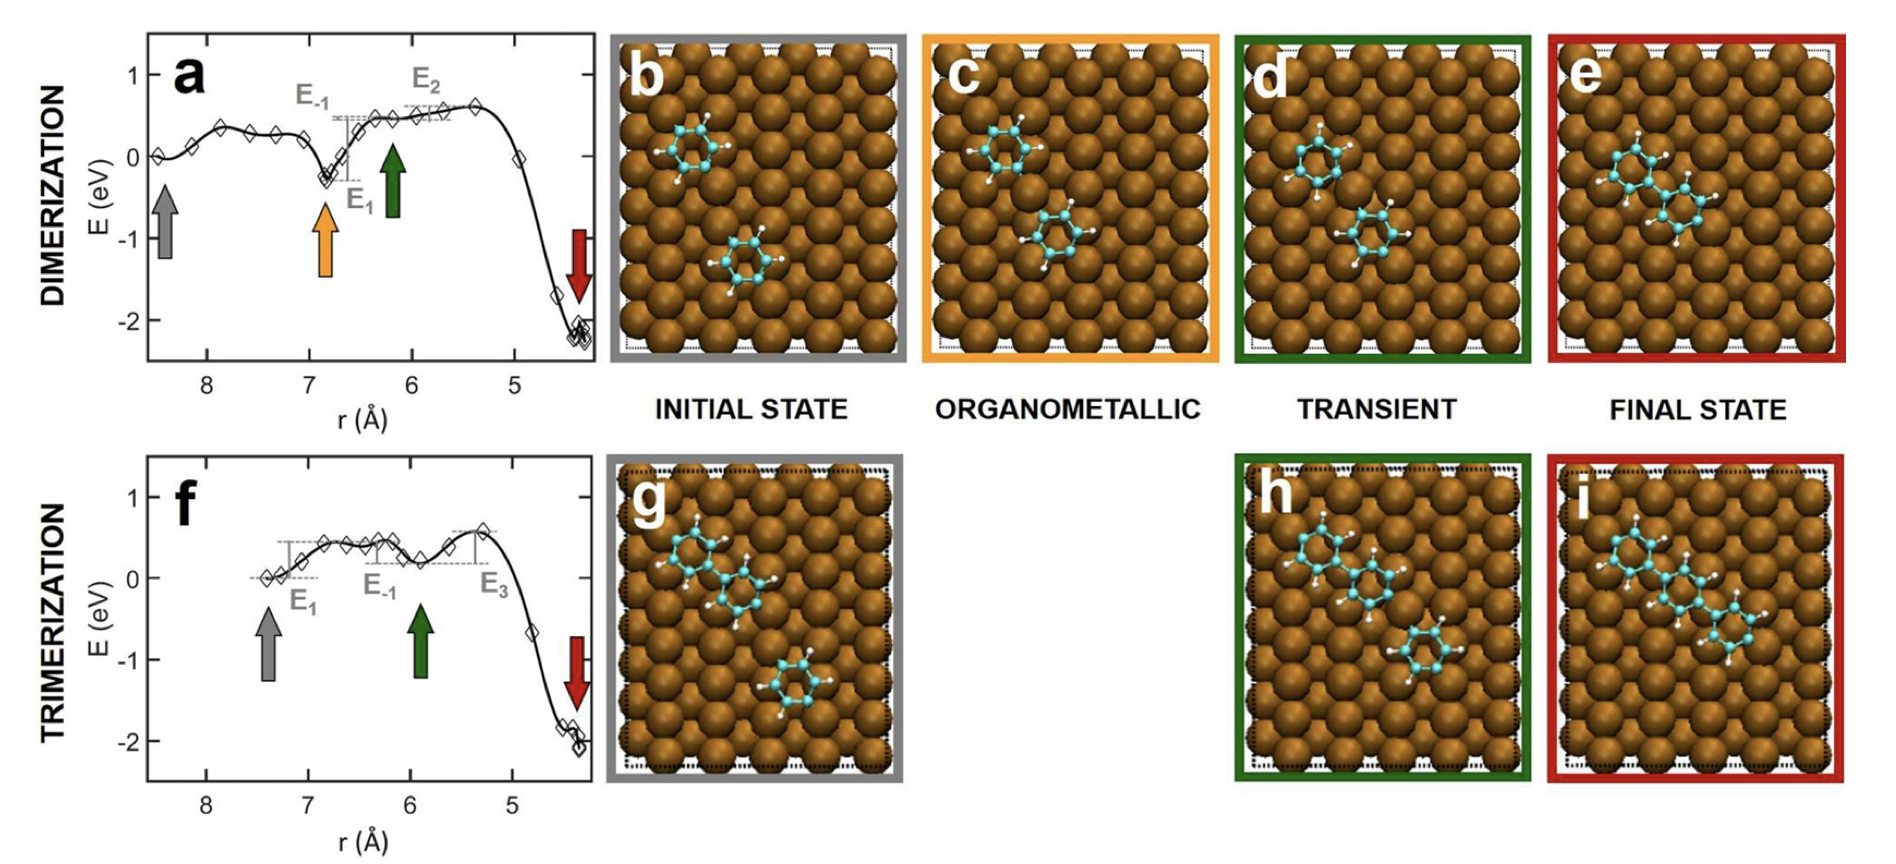
\includegraphics[width=1.0\textwidth]{Fig/Dimer_trimer.png}
%R1111: What metal is this. Better captions are required for all figures. Chemical identity of all species must be clear from the figure.
%\caption{Coupling barriers between (a) two monomers (dimerization) and (f) a monomer and a dimer (trimerization), respectively. The length (r) indicated in angstrom is the distance between the centers of the aromatic rings which undergo covalent coupling. The geometries of the most significant states (initial, organometallic intermediate, transient, and final) are reported in panels b--e and panels g--i for the dimerization and trimerization, respectively. The colors of the frames correspond to the arrows in panels a and f.}
%\label{fig:dimer}
%\end{figure*}
%

%RZK1221: Higher than what?
%RZK1212: Is it important what surface? 111 or other or it does not matter.
This final step requires a higher annealing temperature, ranging from 330 to 420~K on Ag surface and from 500 to 600~K on Au surface~\cite{ullmann_51}. On Cu, the temperature range is usually lower than on Au but higher than on Ag. This indicates that the energy barrier of the formation of C--C bond step on three metal surfaces should follow Au $>$ Cu $>$ Ag. 
%RZK1221: Is it your speculation? If yes, it should be in Results and Discussion. If not, a reference should be given. 
And since there were limited reports on the formation of C-Au-C intermediates, it could be safely speculated that a high energy barrier exists in the formation of C-Au-C dimerized organometallic intermediates and a low barrier exists in the covalent bond formation. 

After the formation of C--C bond, a surface Ullmann coupling would be completed between two monomers, resulting in a dimer. If there are more than one functional groups on a monomer, this dimer could further diffuse and couple to obtain a trimer~\cite{jacs2016}, and oligomers~\cite{ullmann_53, ullmann_56} or polymers~\cite{ullmann_43, ullmann_54, ullmann_55}.


\subsubsection{Summary on mechanism of surface Ullmann Coupling}

{\color{blue}
Overall, the effect of halogens and metal types on each step of surface Ullmann coupling reaction mechanism have been exhaustively explored. 

On dehalogenation step, it has been shown that the reactivity trend decrease in the order Ar--I $>$ Ar--Br $>$ Ar--Cl both in experiment and theoretically~\cite{ullmann_52}. This also means that the dissociation of Ar--I bond on metal surface requires the lowest temperature. In addition, the energy barrier of dehalogenation is the highest on Au(111) surface, the lowest on Cu(111) surface both in experiment and in theoretical calculations~\cite{jacs2013}. It has also reported that the miller index of metal surface will also influence the reaction energy of dehalogenation~\cite{ullmann_57}. 

Then considering the next step, it has been discussed that the diffusion of phenyl group on Au(111) surface is the most energetically favorable, while on Ag(111) is the least. The halogens are supposed to have little influence on the diffusion step, but it might hinder the two phenyl group to diffuse close to each other. 

When it comes to the formation of C--M--C bridge intermediates, it is concluded that C--Au--C structure is the hardest to obtain, the construction of C--Ag--C and C--Cu--C should have close energy barrier due to the similar temperature condition of this step in experiments. 

The covalent bond formation is the last step, different precursors will complete the C--C construction at various annealing temperature on different surfaces. The certain point is this step requires the highest temperature in the whole surface Ullmann coupling procedure.

%RZK1220: What comes next is not relevant to diffusion. Should be discussed in the summary of the mechanism. Or perhaps create a separate subsection "Desorption"
Besides, as we mentioned in the diffusion section that the energy barrier for halogens to diffuse on all metal surfaces are very low, which means halogens may have a high mobility after dissociation. Although halogens are free to move, they possess a relatively high binding energy to metals. The lowest binding energy is halogens on Au(111), around \SI{2.8}{\electronvolt} and the highest is on Cu(111), around \SI{3.1}{\electronvolt}, which indicates that the halogens are even harder to desorb than those dehalogenated phenyl groups. Research also showed that the halogens remained on metal surface will further hinder the diffusion, coupling and polymerization of all kinds of phenyl species~\cite{ullmann_64,ullmann_65}. Removing the byproducts of on-surface Ullmann coupling is also of great significance.

}

\subsection{Role of adatoms in the surface Ullmann coupling} 

%RZK1221: Better introductory sentences about surface defects. 2-3 sentences: types of defects 3D, 2D, 1D.
{\color{blue}
Metal surfaces are not perfect, well-ordered structures. There exists various defects ranging from three-dimensional defect such as pores~\cite{ullmann_72}, cracks~\cite{ullmann_73} to planar defects such as twin boundaries~\cite{ullmann_74}, stacking faults~\cite{ullmann_75} line defects such as dislocations~\cite{Ullmann_76} and point defects such as adatoms~\cite{Ullmann_77}, vacancies~\cite{ullmann_78} shown in Fig.~\ref{cyrstal_surface}~\cite{ullmann_49}. 
%RZK1221: Cite modern review on surface defects, desirably on Cu, Ag, Au. Previously used citation: ~\cite{ullmann_49}

}

{\lock

In the process of the Ullmann coupling, reactants, intermediates and final products interact directly with metal atoms on the surface and, therefore, are affected by surface defects. Quantifying the extent to which imperfections of the metal surface influence the thermodynamics and kinetics of the Ullmann coupling can suggest new strategies for surface optimization, leading, in turn, to higher yields of desirable perfectly-organized [defect-free] two-dimensional polymers. 

\begin{figure}[htb]
\centering
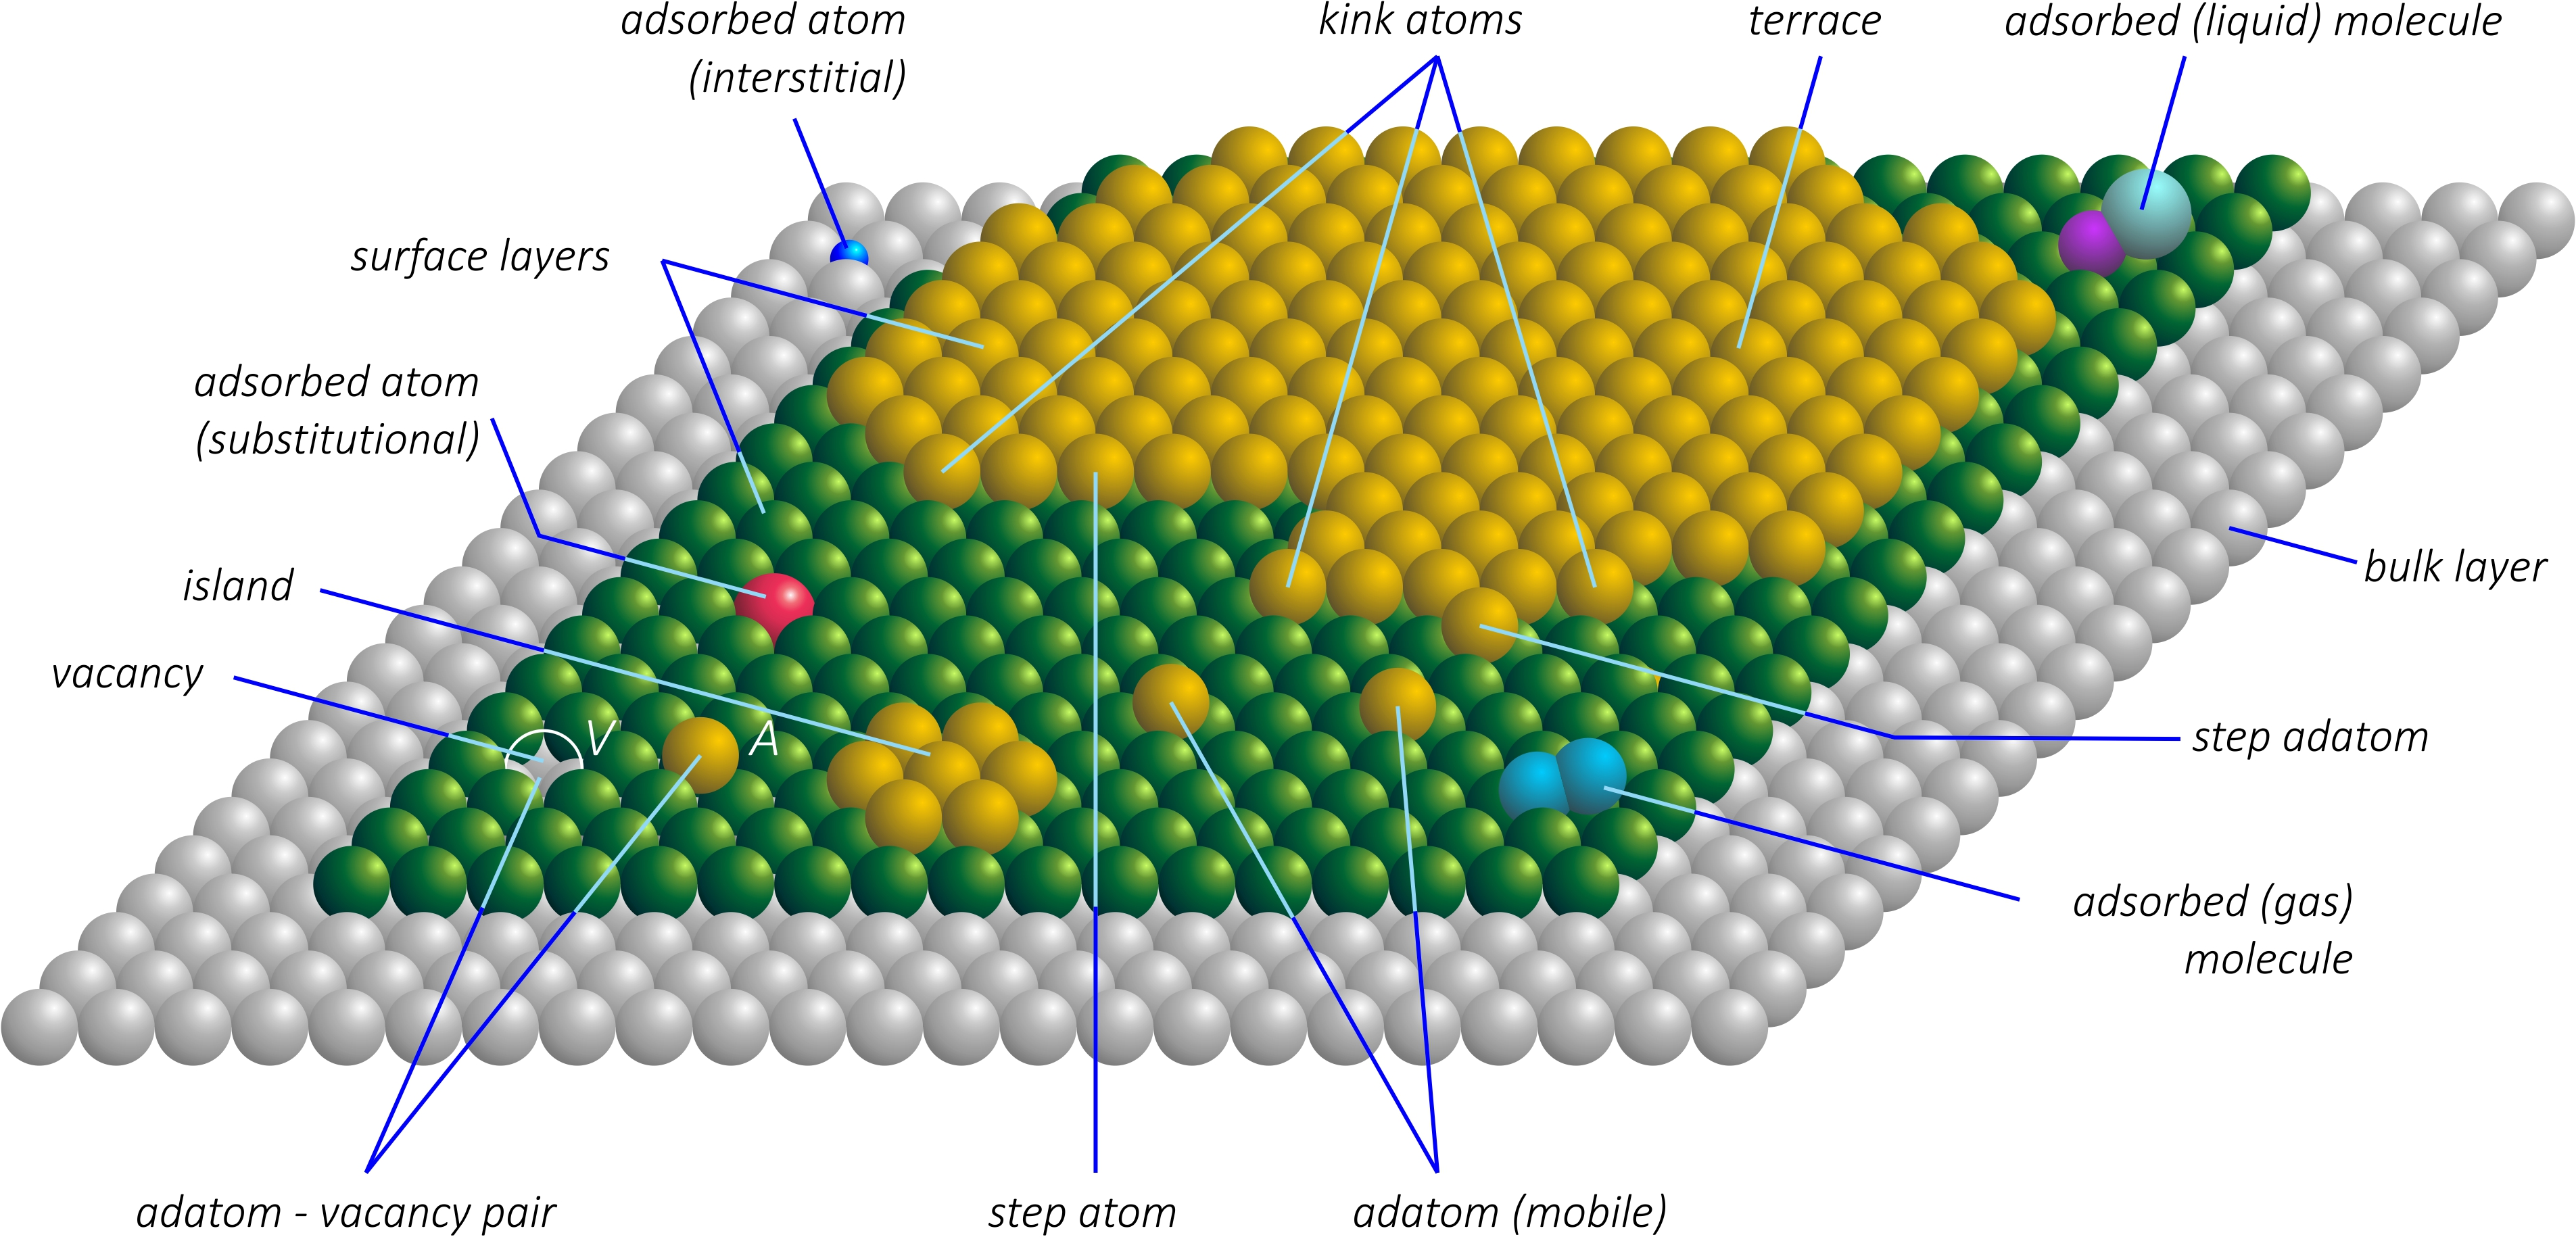
\includegraphics[width=0.4\textwidth]{Fig/Crystal_surface.jpg}
\caption{A model of crystal surface. Adapted from Ref.~\onlinecite{ullmann_49}.}
%RZK1221: Remove the figure or find/create better figure. The text is almost invisible in this figure. 
\label{cyrstal_surface}
\end{figure}

%RZK1221: Do not use math mode to emphasize text. Use \emph{text}.
%RZK1221: The idea to use origin(x) and nature(y) notation is inacceptable. I have never seen anyone doing this in the literature. It makes your text unreadable -- readers will have hard time remembering what your numbers stand for. Go over your text and replace all instances with simple phrases describing your metal atoms.
%nature(1) = ideal-surface atom
%nature(2) = adatom
%origin(1) = pre-existing adatom
%origin(2) = extracted adatom

Surface metal atoms that affect and participate in the Ullmann coupling have different \emph{nature} and \emph{origins}.
Atom's nature describes its immediate environment. Atoms located in the first layer of atoms of the ideal surface will be referred to as \emph{ideal-surface} atoms. \emph{Adatoms}, according to the commonly accepted definition, lie on top of the layer of ideal-surface atoms. In this work, adatoms are differentiated according to their \emph{origin} and can be \emph{pre-existing} and \emph{extracted} adatoms. The origin of pre-existing atoms is irrelevant, not specified, or not known. Extracted adatoms, on the other hand, are known to have been lifted from their lattice sites and placed on top of the surface leaving a surface vacancy behind. In this work, \emph{vacancy} refers exclusively to vacant lattice positions on the surface, not in the bulk.
%RZZK: This section might be better placed into Definitions/Notation part of the manuscript.
%RZZK: The talk about nature and origins is perhaps too formalized. I will simplify it later later.

%%%Here the two terminology $Nature$ and $Origin$ will be used to distinguish the metal atoms which participate in suface Ullmann coupling.
%%%The $Nature$ of metal atoms means metal atoms can come from (1) surface atom which is located at the first layer on metal surface, is indistinguishable from other surface atoms and has no relation with surface defect, or (2) adatoms which is related to the surface defect, it will lie above the first layer of metal surface and free to diffuse.
%%%Thus, the $nature$ mainly divide the metal atoms from a surface into two categories, the first kind is indistinguishable and locate in the lattice of metal crystal, while the second kind is adatoms, which is a production of common non-order defect appeared on metal surface. 
%%%The process that gives birth to $nature(2)$, adatoms in surface Ullmann coupling reaction is also of great interest. It can be split into two different kinds with notation $origin$: adatoms in surface Ullmann coupling may come from (1) pre-exsiting adatoms before the occurrence of surface Ullmann coupling due to the surface defect, thermal punctuation or (2)pulled out by the intermediates produced in surface Ullmann coupling, and then fully sit above the first layer of metal surface to become a new adatom. For the second origin of adatoms, it can also be expressed that the surface Ullmann coupling create this adatom which used to be a $nature(1)$ atom. 

} %lock


{\color{blue}

The nature of metal atoms and the origin of adatoms have been explored experimentally and computationally.
%For origin(1), it has been reported that the onset of the vacancy-adatom formation take place on Cu(111) surface was around 900 K by molecular dynamics~\cite{ullmann_50} , which is much higher than the temperature required by surface Ullmann coupling reaction, as shown in Fig.~\ref{fig:2Dgasn}~\cite{ullmann_50}. This could be the evidence that there would not be new adatoms formation due to the thermal fluctuations as the surface Ullmann coupling proceeds. 

%discuss that adatoms could exit on metal surface due to the thermal evaporation
For \emph{pre-existing} adatoms, it has been explored that Cu adatoms can be released on Cu(111) surface by thermal activation~\cite{ullmann_79, ullmann_58}, silver and gold adatoms can be released on silver and gold surface respectively as well~\cite{ullmann_84, ullmann_85}, especially near surface defects. These adatoms have also been previously observed to
participate in metal organic coordination networks~\cite{ullmann_80, ullmann_81, ullmann_82, ullmann_83}. This coordination phenomena provides a feasible 
possibility that the formation of organometallic intermediates in surface Ullmann coupling can directly make use of \emph{pre-existing} adatoms.
Thus, it can be naturally derived that there is a competition between \emph{ideal-surface} atoms and \emph{adatoms} which actually take part in the structure of intermediates in Ullmann coupling. Also if it is \emph{ideal-surface} atoms that comprise intermediates, these \emph{ideal-surface} atoms can also be fully extracted out from the first layer and become \emph{extracted adatoms}, which can be regarded as an approach to create adatoms on metal surface.
The details of the these arguments are discussed in following sections.

%\begin{figure}[ht]
%\centering
%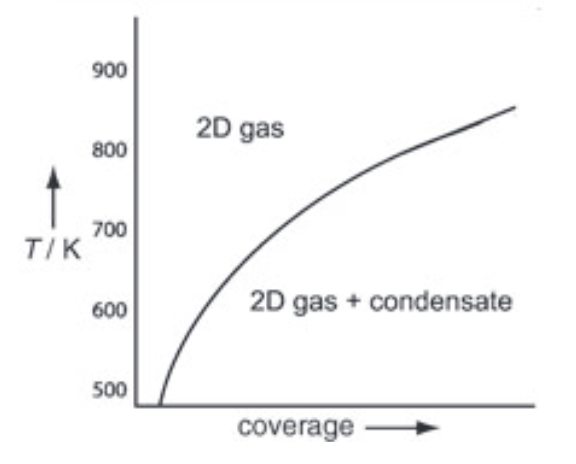
\includegraphics[width=0.75\columnwidth]{Fig/2D-gas.png}
%\caption{Schematic diagram of 2D adatom gas phase and condensed phase (islands) %coexisting at elevated temperatures for metal-on-metal systems.}
%\label{fig:2Dgas}
%\end{figure}


}

\subsubsection{Dehalogenation}

Evidences have already been presented that metal adatoms participate in the process of dehalogenation. 
In 2017, Barton \textit{et al.}~\cite{chemeurope2017} explored the role of adatoms in the dehalogenation step with iodobenzene on Au(111), Ag(111) and Cu(111) surface based on DFT calculations. The energy profile of adatom formation on pristine surface was compared with the profile of formation on surface with the presence of iodobenzene, the latter case is referred to as adatom formation of $origin(2)$. The comparison has shown that the energy of extracting a metal atom from the pristine surface was in the 1.12 - 1.71~eV range. While in the dehalogenation step, the dehalogenated iodobenzene would interact with the metal atom of $nature(1)$ on metal surface, which would possibly form a new adatom of $origin(2)$. This step required a dramatically lower energy of 0.16-0.60~eV range. Furthermore, the calculations have shown that the energy released in the process of adsorption of idobenzene on metal surface and formation of organometallic intermediates in the process of surface Ullmann coupling is sufficient to compensate the energy required for a metal atom extraction to form a new adatom of $origin(2)$, as shown in Fig.~\ref{fig:3}.
\begin{figure}[htb]
\centering
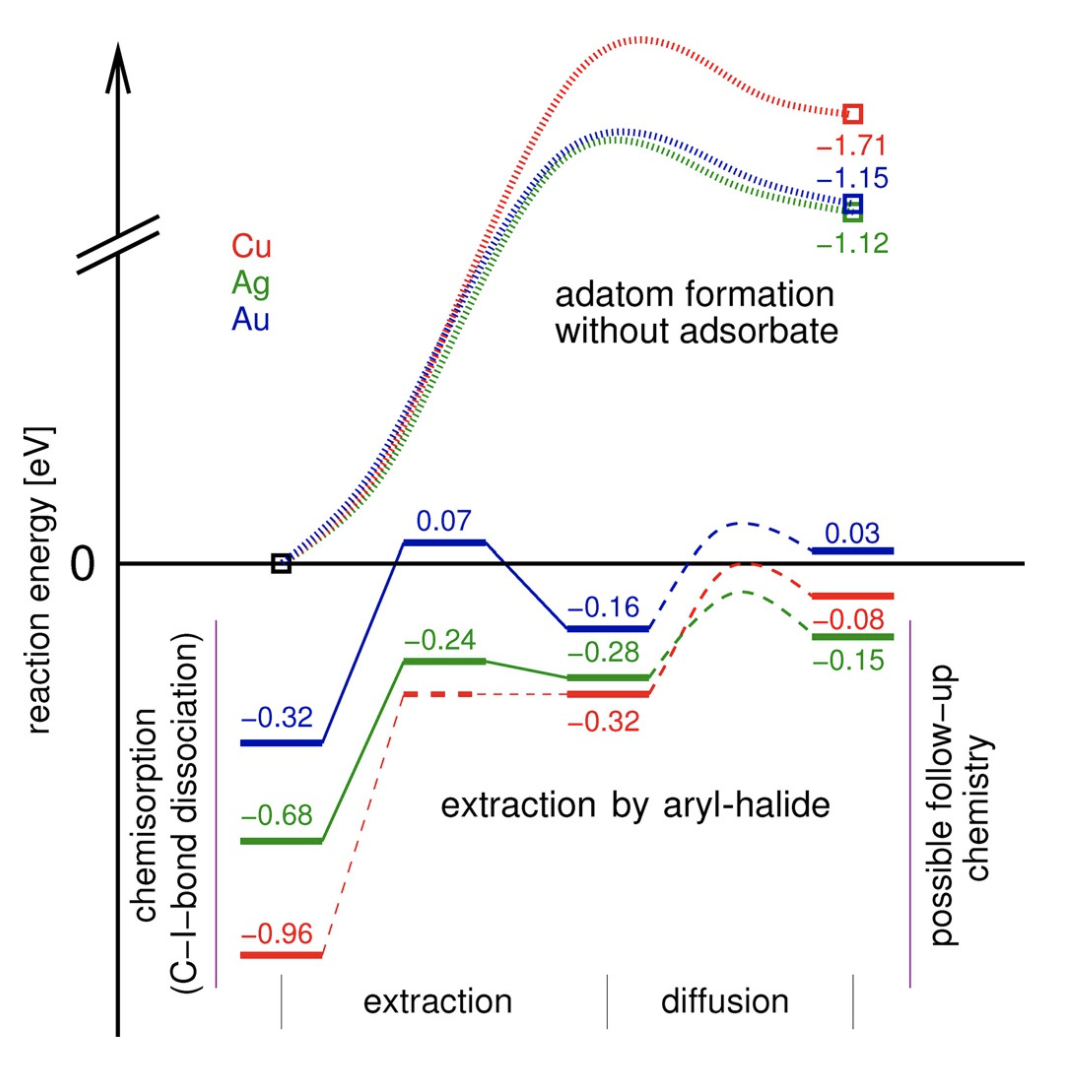
\includegraphics[width=0.75\columnwidth]{Fig/Adatom-formation.png}
\caption{Graphical comparison of the energetics of the adatom formation without adsorbate (top half) to the extraction by aryl–halide process (lower half).Values for Cu are shown in red, for Ag in green and for Au in blue. The extraction-by-arylhalide process starts from the dissociated iodobenzene. Dotted lines indicate parts of the energy profile that have not been quantitatively resolved.}
\label{fig:3}
\end{figure}

It is clear that metal atoms of $nature(1)$ have a great chance to participate in dehalogenation, the first step of surface Ullmann coupling. And the construction of organometallic intermediate in the dehalogenation could possibly be a feasible pathway to form adatom of $origin(2)$. Metal atoms of $nature(2)$ in the dehalogenation had few related reports to date.

{\color{blue}

A multitude of evidences have been presented that metal atoms will participate in dehalogenation as discussed in above section. However, it is still unclear whether \emph{ideal-surface} atoms or \emph{adatoms} are involved in this process. DFT calculations demonstrated that dehalogenation, as the first step of Ullmann coupling, can potentially originate an absolute new adatom by fully extracting an \emph{ideal-surface} atom out from the first layer~\cite{chemeurope2017}. As shown in Fig.~\ref{fig:3}, formation of an adatom on ideal, perfect Cu(111), Ag(111) and Au(111) surface require \SI{1.71}{\electronvolt}, \SI{1.12}{\electronvolt} and \SI{1.15}{\electronvolt} respectively. Dehalogenation of iodobenzene will result in phenyl-metal species, this interaction will decrease the full extraction of \emph{ideal-surface} atom by \SI{1.07}{\electronvolt}, \SI{0.72}{\electronvolt} and \SI{0.99}{\electronvolt} on Cu(111), Ag(111) and Au(111) surface, respectively. The significant reduction in energy indicates that a new adatom can probably be created from an \emph{ideal-surface} atom by organometallic intermediates produced in dehalogenation. 

But it has also been reported that the interaction between single phenyl groups and copper atoms are not adequate enough to fully extract an \emph{ideal-surface} atom out. These phenyl groups produced after dehalogenation will start to diffuse on Cu(111) surface and interact with different \emph{ideal-surface} atoms to form organometallic intermediates~\cite{pccp2010} while all \emph{ideal-surface} atoms involved will stay on their original locations.

Till now it can be concluded that dehalogenation lowers the energy required for creation of adatoms from \emph{ideal-surface} atoms on a metal surface. The direct use of \emph{pre-existing} adatoms should ideally cut down the energy needed for this step compared to \emph{ideal-surface} atoms. However, there are few related work on \emph{pre-existing} adatoms in dehalogenation.



}





\subsubsection{Diffusion}

The diffusion process is involved in the interaction between single precursor group and metal atom. 
In 2018, Nagoya \textit{et al.}~\cite{jpcc2018} investigated the mechanism of Ullmann coupling of 7,10-dibromofluoranthene (Br$_{2}$FL) on Au(111) via DFT calculations. Compared to simple phenyl rings that tend to form ~$36^\circ$ tilt angle with Cu(111) surface~\cite{pccp2010}, the monobromo FL with one Br atom removed would stay almost parallel to Au(111) surface due to steric repulsion between the large backbone of BrFL group and the substrate. And BrFL group was found to lift surface Au atom out by 1.9 \AA\ from its initial position, which is much larger than 0.16 \AA\ height lifted by a simpole phenyl ring, as shown in Fig.~\ref{fig:diff}.
Ebeling \textit{et al.}~\cite{acsnano2019} also indicated 4-bromo-3$^{''}$-iodo-$p$-terphenyl group interacts with the Cu atom inside the surface, and would partially lift the Cu atom out from the surface while diffusing on Cu(111) surface. 
\begin{figure}[hbt]
\centering
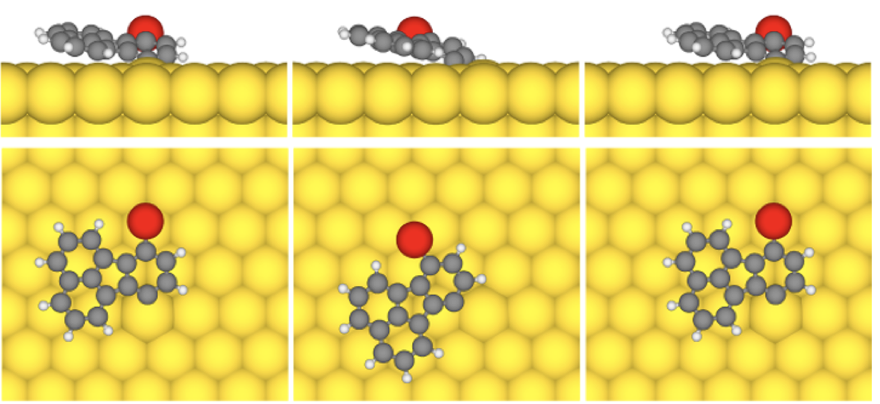
\includegraphics[width=0.75\columnwidth]{Fig/Diffusion_path.png}
\caption{Top and side view of the initial, transition and final geometries of BrFL molecule diffuse.}
\label{fig:diff}
\end{figure}

Metal atoms of $nature(1)$ were proven to play a significant role in the diffusion of dehalogenated phenyl groups, the metal atoms that interact with phenly groups will be partially lifted from its original position, the lifting height is affected by the intensity of interaction between the phenyl group and metal atom. Formation of adatom of $origin(2)$ has not been reported in diffusion, which indicates that the interaction between phenyl group and metal atom in this step is not in the magnitude to fully extract a metal atom of $nature(1)$. 

{\color{blue}

There were no apparent proof that diffusion of dehalogenated species on metal surface can form new adatoms from \emph{ideal-surface} atoms. Most reports were focused on the interaction between the dehalogenated intermediates with \emph{ideal-surface} atoms in diffusion process. The magnitude of this type of interaction is determined by the geometry of intermediates and type of metal atoms.

For single phenyl groups diffusing on Cu(111), it will form \SI{36}{\degree} tile angle with respect to the surface, and the ring structure will flip when it moves between two adjacent copper atoms. Phenly group will lift the \emph{ideal-surface} copper atom by \SI{0.16}{\angstrom} from its original position in diffusion~\cite{pccp2010}. When it comes to the bromofluoranthene molecule diffuse on Au(111) surface, DFT calculation reveals that this aryl group will stay almost parallel to the surface~\cite{jpcc2018}. And the \emph{ideal-surface} gold atom will raise up to \SI{1.9}{\angstrom} from the first layer, \SI{1.74}{\angstrom} higher than phenyl-cooper, owing to the stronger interaction between bromofluoranthene and gold atom.

Whether \emph{pre-existing} adatoms are involved in this step is rarely reported. It can be concluded that diffusion of aryl groups on metal surface can seldom create adatoms since the intensity of interaction between these single dehalogenated species and metal atoms is not sufficient to fully extract \emph{ideal-surface} atoms out.

}

\subsubsection{Formation of C--M--C structure intermediates} \label{sec:dimerized-adatom}

The nature of the metal atoms in dimerized organometallic intermediate has been investigated through multiple approaches. Besides, it can be deduced that an metal atom of $nature(2)$, which is also an adatom of $origin(1)$ will exit above the first layer of surface before the surface Ullmann coupling reacion occurs. And this atom can attract two phenyl groups diffuse close to it and form the dimerized organometallic intermediate in this step. This type of formation might require less energy compared to the situation that two phenyl groups both interact with the same metal atom of $nature(1)$. The arguments on the nature and origin of metal atoms in this step are intense in the mechanism of surface Ullmann coupling.

In 2017, Zint \textit{et al.}~\cite{acsnano2017} analyzed structures of intermediates in the polymerization of bromotriphenylene to bistriphenylene on Cu(111) surface using STM, AFM image and DFT calculations. Two computational models were compared: two triphenylene molecules bonded to an fully-out-of-surface adatom (a metal atom of $nature(2)$) and two precursors bonded to an atom partially lifted from Cu surface (a metal atom of $nature(1)$) as shown in Fig.~\ref{fig:5}. It has been concluded that the structures observed in AFM were more consistent with computational adatom ($nature(2)$) models. In particular, the C--C distance in organometallic intermediate was of 3.9 \AA\ measured by AFM, which was closer to the Cu adatom ($nature(2)$) model (3.86 \AA) compared to the partially-lifted Cu atom ($nature(1)$) model (3.42 \AA). Furthermore, the energy for formation of the adatom-containing intermediate from distant precursors was 1.74~eV lower than that of the intermediate with a partially lifted atoms. 
\begin{figure}[hbt]
\centering
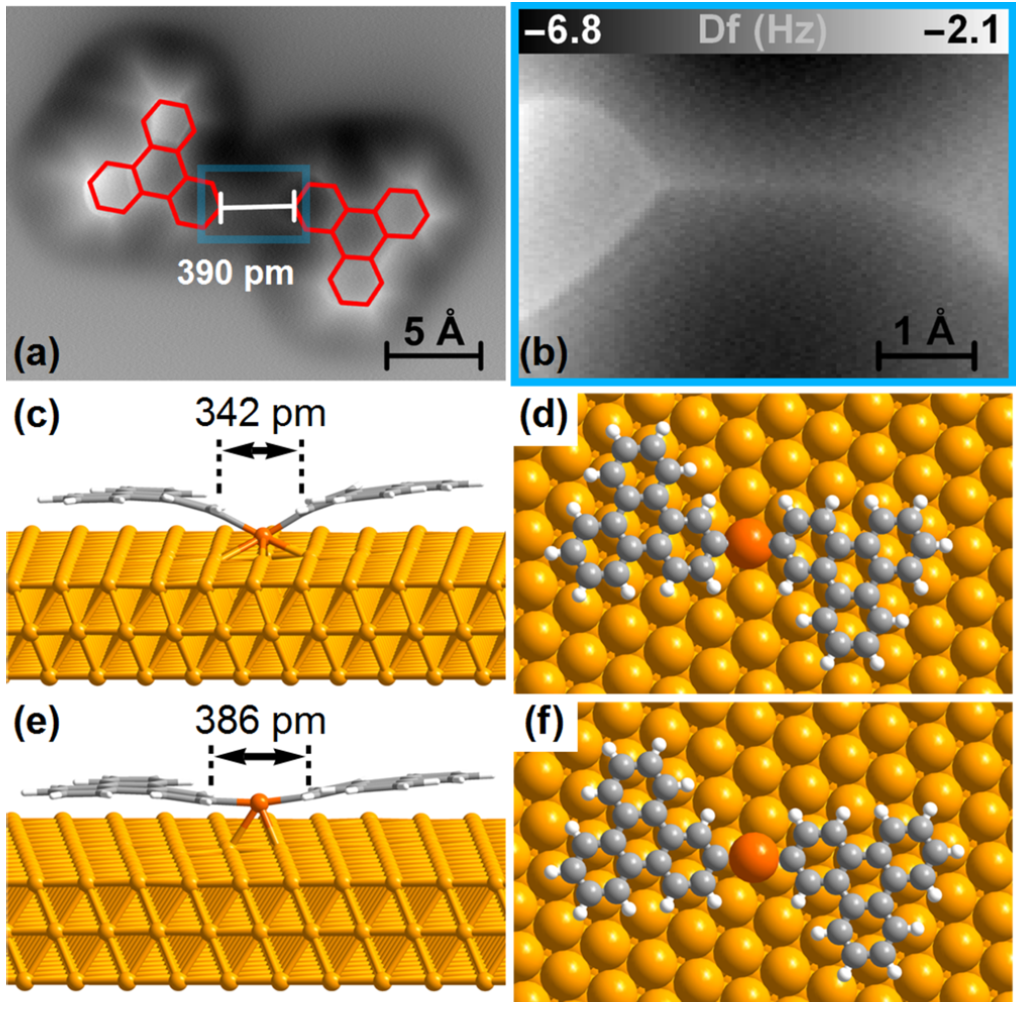
\includegraphics[width=0.75\columnwidth]{Fig/distance.png}
\caption{(a) AFM frequency shift image of intermediate with fit of structural model. (b) Zoom on intermediate bond ($cf$. blue box in a) imaged with decreased tip-sample distance ($\Delta$z = -70 pm with respect to image a). (c--f) DFT-D3 calculations [PBE-D3/ pw (PAW P)] for two different organometallic intermediate states (surface atom (c,d) vs adatom (e,f)).}
\label{fig:5}
\end{figure}

%%ZHZH Dima suggests partial lifting should be discussed separately.
The origin the adatoms were later explored after the metal atoms in dimerized organometallic intermediates were proven to be of $nature(2)$, which is an adatom on surface. In 2019, the study of 4‐Bromo-3$^{''}$- iodo‐$p$‐terphenyl coupling on Cu(111), proved again that the Cu atoms in dimerized organometallic intermediates were adatoms (metal atoms of $nature(2)$) compared experiments with simulated AFM image[Fig.~\ref{fig:6}~\cite{acsnano2019}]. It was further suggested that these adatoms are generated by the extraction of two close single precursor groups (adatom of $origin(2)$), instead of pre-exsiting adatoms (adatoms of $origin(1)$) from a statistic study of all intermediates species in the surface Ullmann coupling.
%
\begin{figure}[ht]
\centering
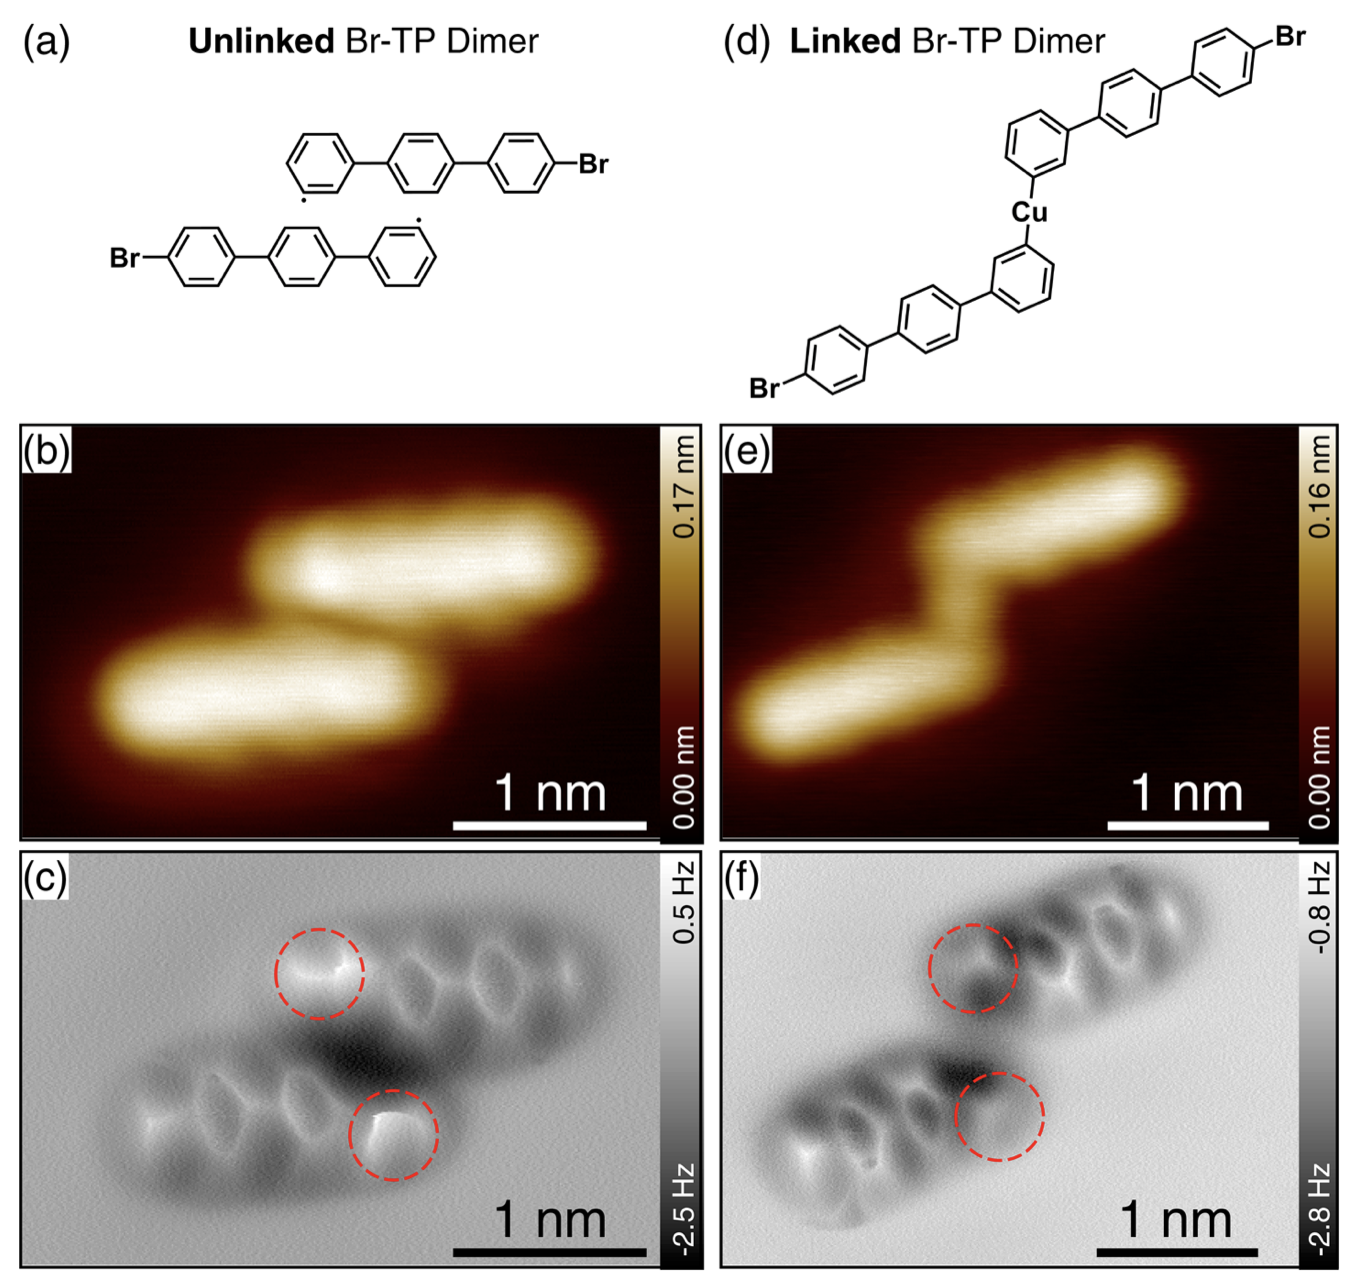
\includegraphics[width=0.75\columnwidth]{Fig/AFM_prove.png}
\caption{Molecular structures (top row), STM (middle row), and AFM images (bottom row) of 4‐Bromoterphenyl dimers on Cu(111). Two different types of dimers are observed, which are denoted as unlinked (left column) and linked dimers (right column). The STM image of the unlinked dimer reveals a dark region between the two molecules that separates them. Between the two molecules of the linked dimer a bright protrusion is observed in the STM scan that directly links them. The red dashed circles in (c) and (f) indicate the twisted phenyl rings, which lost their iodine atoms. Imaging parameters: (b) 200 mV, 30 pA, (e) 200 mV, 10 pA, tip height z = -100 pm (c) and z = -24 pm (f) with respect to a tunneling set point of 200 mV and 10 pA on Cu(111).}
\label{fig:6}
\end{figure}

The nature of metal atoms in dimerized organometallic intermediates has been proven to be an adatom. And further the origin of this adatom is of $origin(2)$, which indicates before the surface Ullmann coupling reaction occurs, the adatom is still a metal atom of $nature(1)$, stay in the first layer of metal surface. After it was selected from two phenyl groups in coupling procedure, it will be fully lifted out of the surface, become a new adatoms. The effect of metal atom in the last step --- formation of C--C bond was not investigated intensive compared to previous steps.

%In addition, chlorinated prophyrin as precursor has also been deposited on Cu(111)~\cite{chematerial2019}. Based on DFT calculations, the Cu adatom mediated path is 3~eV lower than the direct dechlorination. And from STM image, some precursors are still intact at temperature of 400~K, which should be already dehalogenated at lower temperature. It proves that the Cu adatoms are the limiting agent [Fig.~\ref{fig:prophyrin}].

%\begin{figure}[ht]
%\centering
%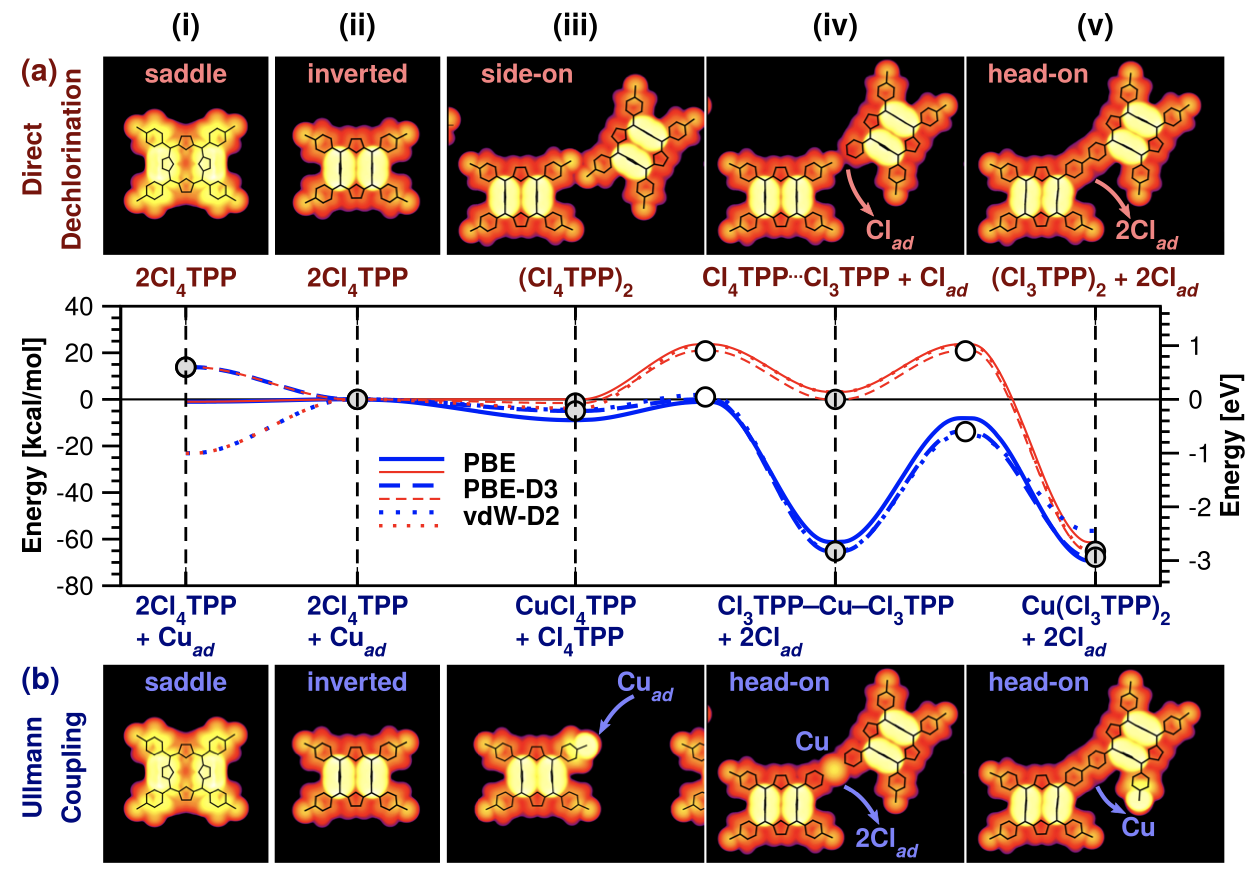
\includegraphics[width=0.4\textwidth]{Fig/Complete.png}
%\caption{STM simulations and DFT reaction profile for the (a) direct %dechlorination reaction (red lines) and (b) Cu adatom-mediated Ullmann coupling reaction (blue lines). For each process the energy are plotted of the (i, ii) precursors, (iii, iv) intermediates, (v) and final species (gray circles) and two transition states (white circles).}
%\label{fig:prophyrin}
%\end{figure}

{\color{blue}
The mechanism of metal atoms participating in the formation of C--M--C bridges structure are most intensively investigated among all other steps in surface Ullmann coupling. Multiple approaches have been used to figure out it is \emph{adatoms} or \emph{ideal surface} atoms that actually constitute the C--M--C bridge. 

DFT calculation results state that two phenyl groups, after diffusing to adjacent position, will bind to the same \emph{ideal surface} copper atom and form C--Cu--C structure on Cu(111)~\cite{pccp2010}. Similar structure will be constructed on Ag(111) and Au(111) surface from phenyls and \emph{ideal surface} silver and gold atoms.

However, disagreement has been proposed with other precursors. Fig.~\ref{fig:5} describes the process that two triphenylene groups with a copper atom form a C--Cu--C structure on Cu(111) surface using AFM and DFT methods~\cite{acsnano2017}. Two distinct simulation models are shown: (1) the copper atom in C--Cu--C structure comes from \emph{ideal surface} atom as shown in (c) and (d). This \emph{ideal surface} atom is partially lifted up from it original position in the first layer of metal; and (2) the copper atom in C--Cu--C is an \emph{adatom} as pictured in (e) and (f). Two model are compared with AFM image on atomic properties. The distance between carbon and carbon in this C--Cu--C bridge in AFM, \emph{ideal surface} model and \emph{adatom} model are \SI{3.90}{\angstrom}, \SI{3.42}{\angstrom} and \SI{3.86}{\angstrom} respectively, which proves that the \emph{adatom} model is more consistent with the molecule geometry in experiment. In addition, the energy required to form the C--Cu--C bridge structure from these precursors with \emph{adatom} is estimated to be \SI{1.74}{\electronvolt} lower than with \emph{ideal surface} atom. The metal atoms in C--M--C intermediate structure were proven to be adatoms with clear evidence for the first time. Then the pathway of emerging such adatoms was also reported.

In Fig.~\ref{fig:6}, the STM and simulated AFM image of forming C--Cu--C intermediate structure from 4‐bromoterphenyl and copper atom are displayed~\cite{acsnano2019}. Based on the comparison of the experimental STM and simulated AFM image data, the metal atom participated in the C--Cu--C structure is again, proven to be adatoms. Furthermore, these adatoms, according to the statistic data, are created during the surface Ullmann coupling reaction by extracting the \emph{ideal surface} atoms out instead of \emph{pre-existing} adatoms before the coupling process.

In this step, the confusion on the origin of metal atoms is approaching to be clear. Previously works suggest that the metal atoms in C--M--C intermediate structures are most likely to be adatoms. And the formation of such a bridge structure is expected to be a feasible strategy to create adatoms on Cu(111) surface. However, as discussed in former section, the intensity of interaction between aryl groups and metal atoms will be determined both by the molecule geometry of aryl group as well as the type of metal atoms. Whether surface Ullmann coupling of all possible precursors on different surfaces will obey the same mechanism still remains adequate space for further exploration and discussion.

The  effect  of  metal  atoms  in  the  last  step  —  formation of C-–C bond was not investigated widely compared to previous steps.
}


\subsection{Objectives}

{\lock
%RZK1223 I will write this one.

The focus of this work is on the role of adatoms in the surface Ullmann reaction, exemplified by the coupling of two phenyl rings -- one of the most studied and simple model of the Ullmann process.

%RZZK: Further limitations of this article.
Cu(111). Three halogens.

%RZZK: as well as the microscopic mechanisms of interaction of all species with various defects, energy profile

}

\section{Methods}
%\subsection{Computation Models}

\subsection{Computational Details}

%RZK: learn how to use si package and correct all units here.
The periodic density functional theory calculations were performed using the Perdew–Burke-Ernzerhof (PBE) for the exchange-correlation functional, the projector augmented wave method for the ion-core electron interactions, and a plane-wave basis set as implemented in the Vienna ab-initio simulation package (VASP) code. Van der Waals (vdW) interactions were included using the DFT-D3 method to describe the nonlocal correlation energy. 

The Cu(111) surface used in all surface Ullmann coupling was 
modeled by a four-layered slab consisting of 192 Cu atoms (a p($48\times 4$) unit cell) and at least 15~\AA of vacuum. The relaxations were performed with applying spin-polarization. The energy cut-off for the plane-wave basis was set to 800 eV and a $3\times 3 \times1$ k-mesh was adopted. The mesh density of k points was kept fixed in related calculations with primitive cells. All atoms were fully relaxed until the MAX force on the atom was less than $2\times 10^{-2} eV/\si{\angstrom}^{2}$. 

Transition-state calculations were carried out using a Climbing-Image Nudged Elastic Band (CI-NEB) methods with VTST code\cite{ullmann_59}. An improved initial guess~\cite{ullmann_60} for minimum energy path was conducted in CI-NEB calculation, different number of intermediates were interpolated between the initial and final configurations due to the distance between them. Plus, All atoms were fully relaxed until the MAX force on the atom was less than 0.1~\si{\eV\square\angstrom} in CI-NEB calculations.

Generally the value of most thermodynamic functions can be derived from our DFT optimization results. 
(%ZZ1215: still miss the math part, will add later)

The simulation of surface Ullmann coupling reaction was conducted with chlorobenzene, bromobenzene and iodobenzene on Cu(111) surface. We explored the mechanism discussed above step by step including the least reported step --- formation of C--C bond.

In the dehalogenation step, the CI-NEB method was used in chlorobenzene, bromobenzene and iodobenzene precursors to study how different halogens will affect on the dissociation of carbon-halogen bonds. CI-NEB method offered us energy profile diagram as well the transition state.

\section{Results and Discussion}

\subsection{Physisorption}

{\lock

The precursors of surface Ullmann coupling are physisorped on the Cu(111) surface before the initialization of the chemical process. The calculated adsorption energies are -1.06~eV, -1.18~eV and -1.37~eV for chlorobenzene, bromobenzene and iodobenzene, respectively. 

} %lock

%RZK1223: Numbers from previous calculations. What computational methods have been used before?


\subsection{Dehalogenation}

%RZK1223: We do not seem to need this energy at this point.
%(In the literature, they mentioned that in the gas phase, the dissociation reaction are highly endothermic (3.85 eV for bromobenzene and 3.33 eV for iodobenzene), we can get the energy for this reaction too)

Fig.~\ref{fig:dissociation_Cl}, Fig.~\ref{fig:dissociation_Br} and Fig.~\ref{fig:dissociation_I} shows the initial, transition and final states (notated as IM1, TS1 and IM2 in Fig.~\ref{fig:completeenergy}, respectively) of chlorobenzene, bromobenzene and iodobenzene dehalogenation on Cu(111), respectively. 

RZK: First state reaction energies. Negative energies already mean that the reaction is exothermic, there is no need to state this.

Dehalogenation reactions of three precursors are all exothermic, which in reverse, are endothermic in gas phase according to the DFT calculated energies. This is due to the formation of energetically unstable radical in gas phase, but copper surface can donate electrons to stable these intermediate species.
%R1111: Do you mean our calculated enthalpies or experimental values? (%ZZ: add descriptions)
%R1111: Why your state lalbels (IM2, IM1) disagree with those in the final energy profile?(%ZZ: changed)
The energy change ($\Delta E$ = $E_{IM2} - E_{IM1}$) of dehalogenation of chlorobenzene, bromobenzene and iodobenzene on Cu(111) are -0.58 eV, -0.8 eV and -0.94 eV, respectively. As seen from the Figures~\ref{fig:dissociation_Cl}--\ref{fig:dissociation_I}, the halogens always occupy the hollow site of Cu(111) surface after the carbon-halogen bond (C-X) is broken. 
%R1111: Physisorption must be described before dissociation. Negative, not positive adsorption energies must be used
In IM1, the precursor molecule was physisorbed by the surface, the adsorption energy are 1.06 eV, 1.18 eV and 1.37 eV, respectively for chlorobenzene, bromobenzene and iodobenzene. (%ZZ: added)
%
In the TS1, the geometry of chlorobenzene, bromobenzene and iodobenzene on Cu(111) are similar, forming a tilt angle, ready for the break of C-X, the distance of C-X are 2.18 \AA\, 2.46 \AA\ and 2.61 \AA\, respectively. 
%R1111: Report bond elongations, not only bond lengths.
After dehalogenation, the phenyl species and halogen atoms were separately chemisorbed by Cu(111) surface. In IM2, the distance between the carbon and halogen are increased by 1.81 \AA\, 1.64 \AA\ and 2.49 \AA\ compared to original distance, respectively. The geometry of IM2 for chlorobenzene, bromobenzene are similar, in which the phenyl species displayed a more tilt angle with the copper surface compared to the TS1. 
%R1111: Compare you results to Ph-I in barton2017fromation (Figure5-Cu_IS in their article). They do not have vertical position for the phenyl.  (%ZZ: recalculated, the first time still vertical, try to change to initial geometry)
However, In the TS1 of iodobenzene, the phenyl specie is almost vertical to the copper surface. This makes a contribution to the highest enthalpy of iodobenzene dehalogenation. Another reason why iodobenzene possesses the highest enthalpy may come from the strongest chemisorption of Iodine on Copper. 
%R1111: Do we want to perform additional calculations to figure out the reason? Perhaps not now. (%ZZ: agree)

%R1111: The first sentence is trivial and must be removed. Do not define energy barrier in Results section. This definition is trivial and can be omitted.
Secondly, the $E_{barrier}$ ($E_{barrier} = E_{TS1} - E_{IM1}$) for three halogenation reaction were also computed and summarized, which are 1.25 eV, 0.92 eV and 0.68 eV, for C-Cl, C-Br and C-I respectively. These $E_{barrier}$ values indicate that the carbon-iodine bond is the easiest to break on Cu(111) surface while the carbon-chlorine bond is the hardest. This is consistent with the experimental data that most carbon-iodine and carbon-bromine bonds will dissociate at room temperature, but an higher temperature is required to break carbon-chlorine bonds in surface Ullmann coupling. The $\Delta E$ and $E_{barrier}$ were also computed in Björk's ~\cite{jacs2013} work. $\Delta E$ were -0.70 eV and -0.82 eV and  $E_{barrier}$ were 0.72 eV and 0.40 eVfor bromobenzene and iodobenzene on Cu(111). Trends are the same with our results, the difference between specific values may come from their use of different functional (optB86b) and the size of slab (four layers 6x6).

%R1111: Some of these findings have been reported in the literature before. Comparison to previous calculations is necessary. "Trends are the same but numbers differ. Why? Do they use the same XC functional, basis set?" (%ZZ: added)

Summarizing the dehalogenation results, the reaction mechanism of chlorobenzene, bromobenzene and iodobenzene are very comparable on Cu(111) surface, the geometry of TS1 are analogous. The phenyl species of chlorobenzene, bromobenzene form a tilt angle with Cu(111) surface and it is vertical for iodobenzene. The dehalogenation of iodobenzene is the easiest among these three reactions due to the lowest activation energy.

%R1111: All figures must be formatted to make text readable. It might be desirable to place all profiles into one figure. 
\begin{figure*}[hbt]
\centering
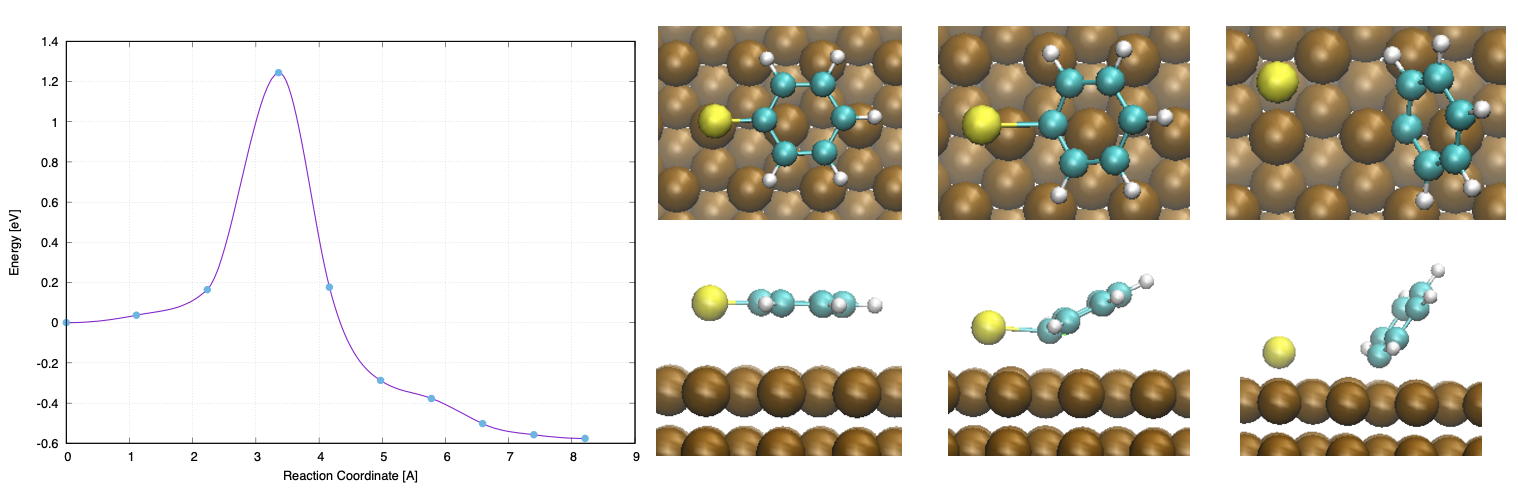
\includegraphics[width=1.0\textwidth]{Fig/dissociation_Cl.png}
\caption{The dissociation of C-Cl bond on Cu(111) surface, left is the energy diagram of the CI-NEB calculations, right side are the top and side view of $IS$, $TS$ and $FS$. (Sphere with ochre color is copper atoms, with cyan color is carbon atoms, with white color is hydrogen atoms. Same in below models. Sphere with yellow color is chlorine atom)}
\label{fig:dissociation_Cl}
\end{figure*}

\begin{figure*}[hbt]
\centering
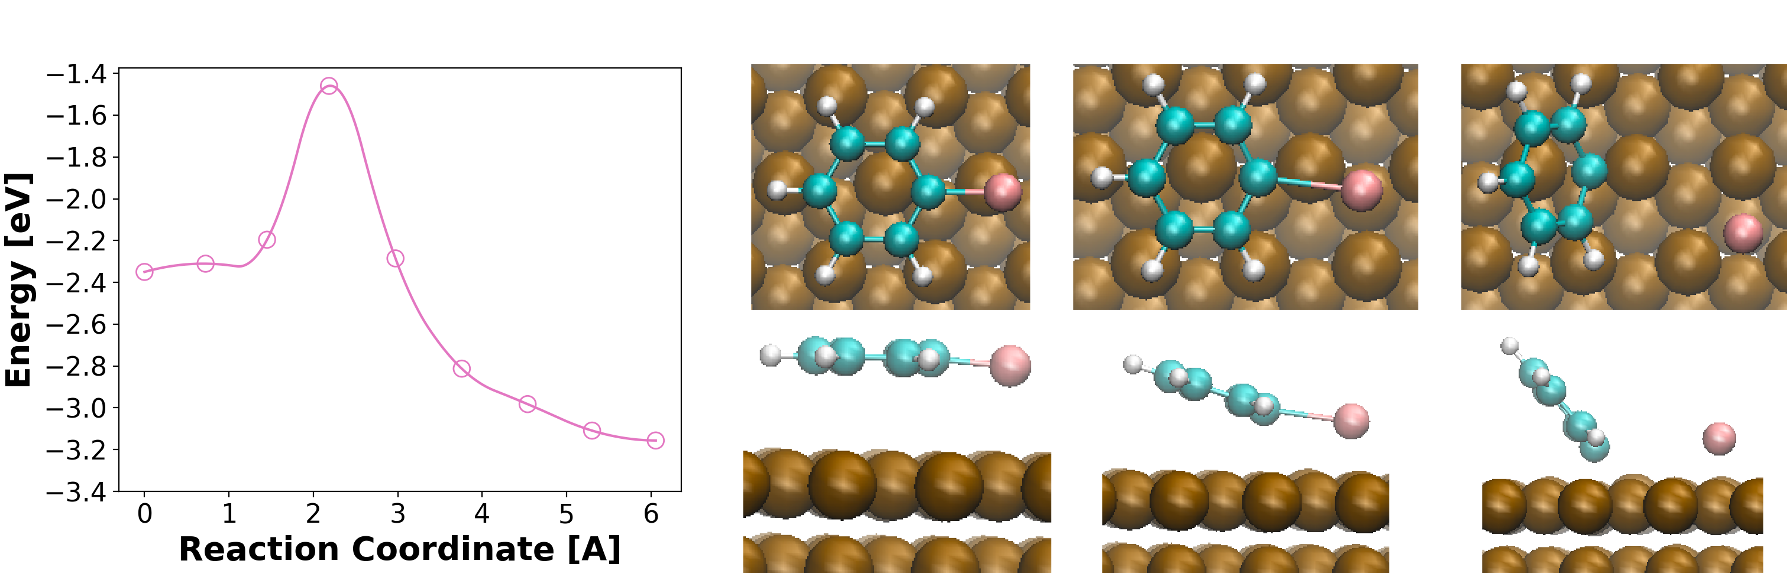
\includegraphics[width=1.0\textwidth]{Fig/dissociation_Br.png}
\caption{The dissociation of C-Br bond on Cu(111) surface. (Sphere with lime color is bromine atoms)}
\label{fig:dissociation_Br}
\end{figure*}

\begin{figure*}[hbt]
\centering
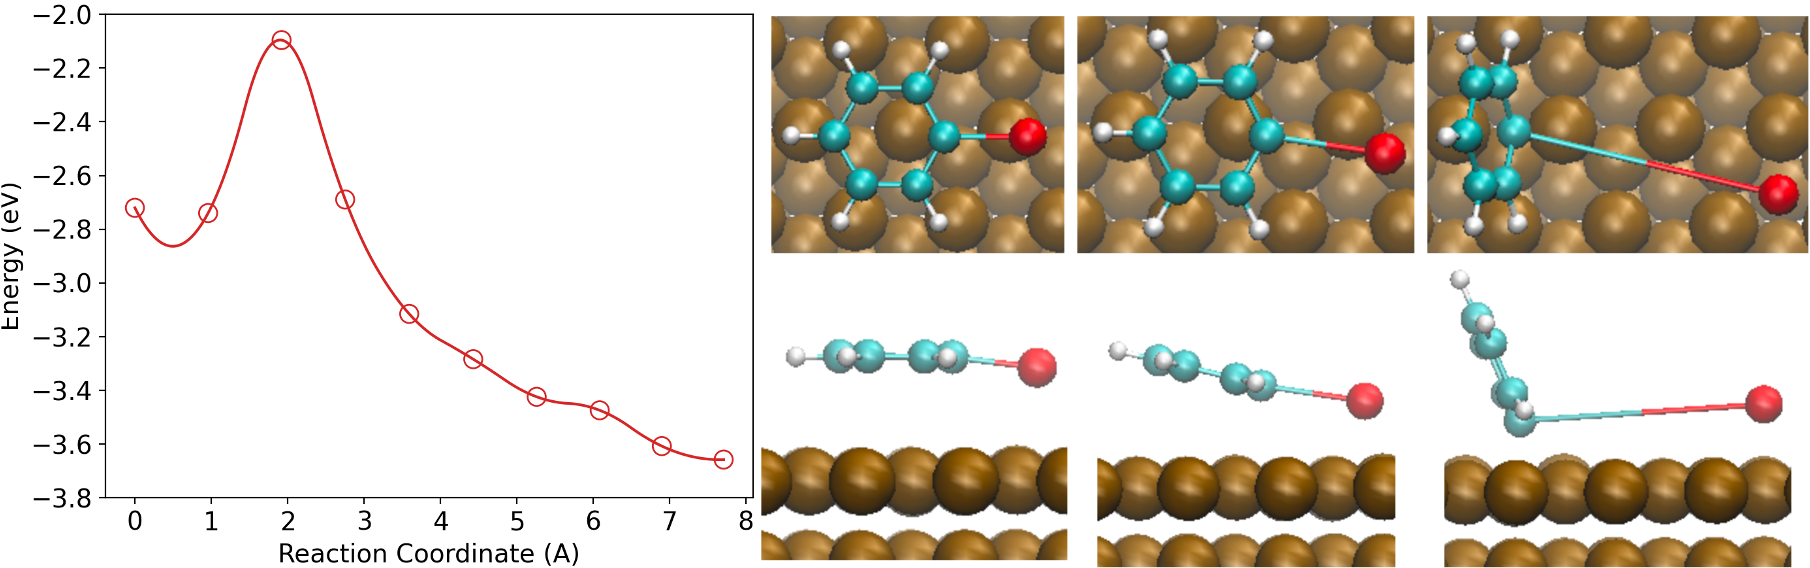
\includegraphics[width=1.0\textwidth]{Fig/dissociation_I.png}
\caption{The dissociation of C-I bond on Cu(111) surface. (Sphere with red color is iodine atoms)}
\label{fig:dissociation_I}
\end{figure*}

\subsection{Diffusion and Formation of Dimerized Organometallic Intermediates}

%R1111: do not use "would". State facts with certainty. "To for a C--C bond the diffusion MUST brings two phenyl groups together." (%ZZ: ok)
After the dehalogenation, the diffusion of all species on copper surface must bring two orientation-matched phenyl groups together, leading to the formation of dimerized organometallic intermediates. Since the halogens such as chlorine, bromine and iodine have been dehalogenated and then chemisorbed by the surface, these three different precursors can be fairly considered to form the same dimerized organometallic intermediate structure in this step.

Fig.~\ref{fig:organometallicintermediate} shows the optimized geometry of dimerized organometallic intermediate on Cu(111) surface. From the left picture, it is apparent that these two phenyl groups both conducted interactions with the copper atom on Cu(111) surface; from the right side, it shows that, the copper atom that interacted with two phenyl groups is partially lifted from the first layer flat. This metal atom belongs to $nature(1)$. And this phenomenon does not take place when there is only one phenyl group since the interaction is not strong enough. 

%R1111: Why chlorobenzene is so different? Halogen does not participate in this step at all. How come that the reaction energy is so different?
Besides, the energy change of the reaction for three precursors from dehalogenated chlorobenzene, bromobenzene and iodobenzene to dimerized organometallic intermediate are +1.40 eV, +0.17 eV and +0.17 eV, respectively. These three reactions are all endothermic, and the dehalogenated chlorobenzene will adsorb the most energy, which is consistent with the experiment that transformation to dimerized organometallic intermediates from dichlorobenzenes wound not be completed unless a higher temperature is present, but transformation of dibromobenzenes and diiodobenzenes would fulfill at room temperature.

%R1111: It looks like this unfinished paragraph belongs to the next subsection: formation of the C--C bond.
Here, we considered that the dimerized organometallic intermediates were formed with the copper atom of $nature(1)$. In reality, the copper atom in organometallic intermediates may also come from the adatom which is of $nature(2)$. It will lay above the surface before the coupling reaction occurs. In this case -----

%R1111: This intermediate is shown in the figure for the C--C bond formation. Remove this figure, re-reference.
%\begin{figure}[hbt]
%\centering
%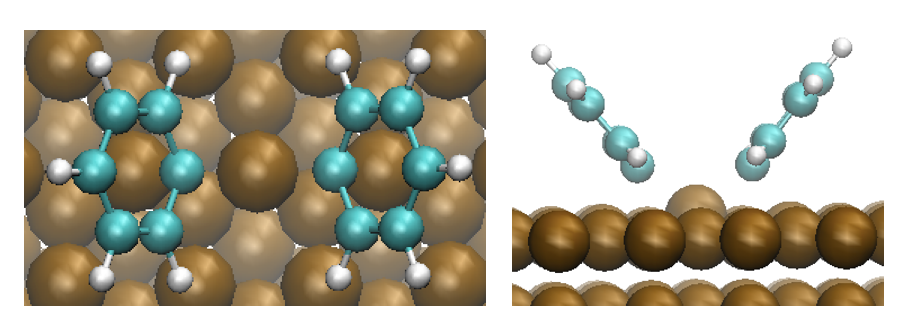
\includegraphics[width=0.45\textwidth]{Fig/organometallicintermediate.png}
%\caption{The organometallic intermediate on Cu(111) surface}
%\label{fig:organometallicintermediate}
%\end{figure}

\subsection{Formation of Carbon Carbon (C--C) Bond}

The final coupling step is the formation of carbon carbon bond (C--C). As discussed above, we explored the two pathways of the C--C bond formation starting from  the Cu atom partially lifted from the surface by two phenyl groups. In the first pathway (Path~1), the Cu atom returns back to its original position in the first surface layer once the C-C bond is formed without producing an adatom. In the secind pathway (Path~2), the Cu atom is pulled out from its original position to become an adatom and leaving the vacancy in its original position. %This means that the metal atom is of $nature(1)$ at the beginning of surface Ullmann coupling, and in the end it changes to $nature(2)$ through the $origin(2)$ method, becoming a new adatom on metal surface.
Here, we investigated two possibilities separately.

\subsubsection{Path I: Cu Returns to Original Location after Coupling Reaction}

%R1111: LATER. We need to develop better notation for all chemical species and refer to them consistently.
%R1111: comparison to existing calculations. Comparison between different metals (and halogens?) in our own calculations.
In Path I, the formation of C--C bond started from the dimerized organometallic intermediate in which the copper atom was partially lifted (notated as $IS_{path1}$). Then the two carbons which would construct a new bond later slope closer to each other, while the copper atom was less lifted on the surface (notated as $TS_{path1}$). Finally, a new C-C bond was formed and the surface went back to original configuration, no adatom forms after the coupling reaction finished (notated as $FS_{path1}$).

%In Fig.~\ref{fig:bondformlift}, along the potential energy surface, 6 intermediates were interpolated between $IS_{path1}$ and $FS_{path1}$. The tilt angle of phenyl species in respect to the Cu(111) surface was $50^\circ$ in $IS_{path1}$ and flattened to $35^\circ$ in $TS_{path1}$ and ended at $0^\circ$ in $FS_{path1}$. The distance between the two carbon atoms which would construct a bond varied from 3.10~\si{\angstrom} to 2.28 \AA\ and ended at 1.49 \AA\.

In Fig.~\ref{fig:bondformlift}, along the potential energy surface, 6 intermediates were interpolated between $IS_{path1}$ and $FS_{path1}$. The tilt angle of phenyl species in respect to the Cu(111) surface was 50\si{\celsius} in $IS_{path1}$ and flattened to $35^\circ$ in $TS_{path1}$ and ended at $0^\circ$ in $FS_{path1}$. The distance between the two carbon atoms which would construct a bond varied from 3.10~\si{\angstrom} to 2.28~\si{\angstrom} and ended at 1.49~\si{\angstrom}.

Path I reaction is exothermic, the enthalpy $\Delta H$ is -2.00~\si{\eV}, and $E_{barrier}$ is 0.50 eV.
%R1111: This results agree with the computational study of the C--C formation of dibromobenzene species. Reference.

%R1111: LATER. It is important to discuss the zero-energy for this step. Would it be more informative to use a common zero from the entire energy profile?
\begin{figure*}[hbt]
\centering
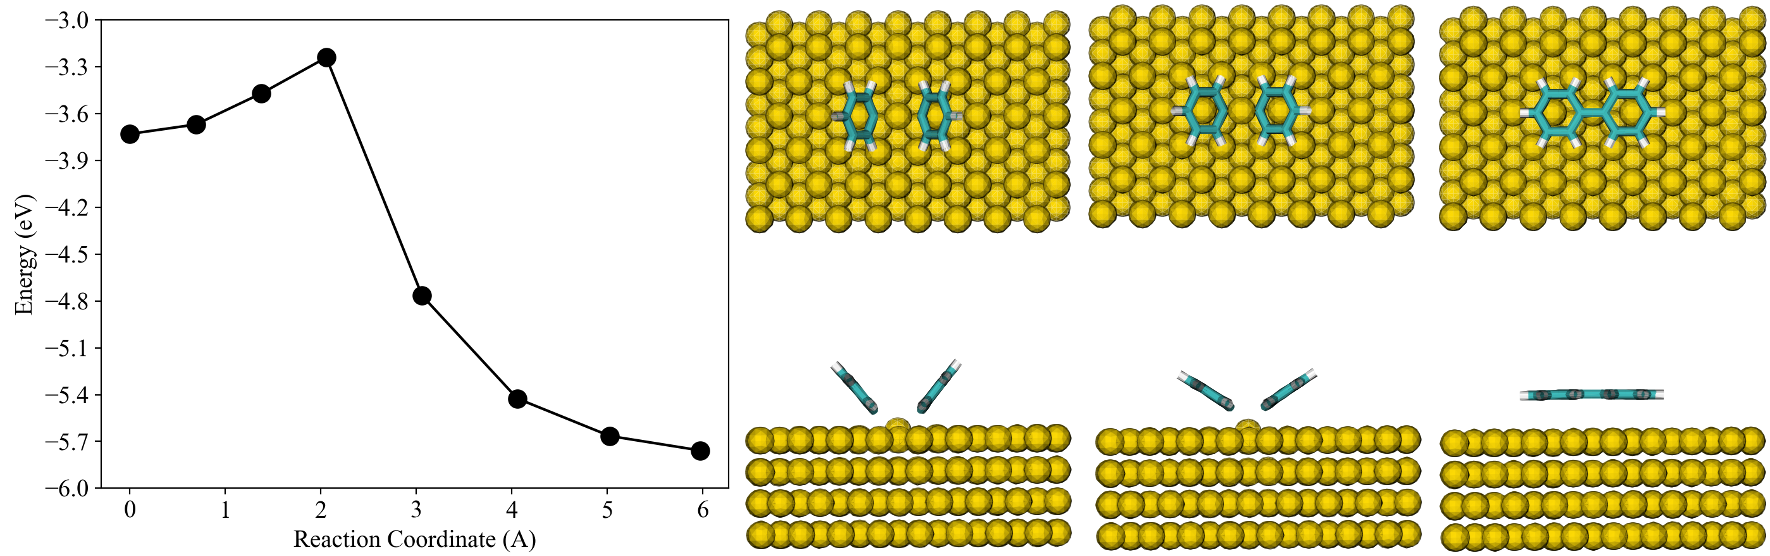
\includegraphics[width=1.0\textwidth]{Fig/bondformlift.png}
\caption{C-C bond formation through lifting Cu atom Path I}
\label{fig:bondformlift}
\end{figure*}


\subsubsection{Path II: Cu becomes a new adatom after coupling reaction}

In Path II, the process started from the organometallic intermediate whereh the copper atom is fully pulled out as an adatom (notated as $IS_{path2}$) (here we created a vacancy on surface corresponding to the creation of adatom, to assure the whole system has the same number of atoms). Then the two phenyl groups would be lifted higher and closer to each other, while the copper atom is less lifted and move towards a hollow site on the surface(notated as $TS_{path2}$). Finally, a new C-C bond is formed and a new adatom and a new vacancy are created on the surface (notated as $FS_{path2}$).

As Fig.~\ref{fig:bondformadatom} show, in this path, 10 intermediates were interpolated between $IS_{path2}$ and $FS_{path2}$.The tilt angle of phenyl species in respect to the Cu(111) surface initialized at $8.5^\circ$ and $12.2^\circ$ in $IS_{path2}$ (the difference angle could be accounted by the fact that vacancy is close the one phenyl species, this will affect a little on the tilt angle), then flattened to nearly $0^\circ$ in $TS_{path2}$ and ended at $-9.1^\circ$ in $FS_{path2}$ (the negative angle arises from the fact that the adatom is right behind the biphenyl). The distance between the two carbons which would construct a bond varied from 3.89 \AA\ to 2.53 \AA\ and ended at 1.50 \AA\ .

Path II reaction is slightly exothermic, the enthalpy $\Delta H$ is -0.17 eV, and $E_{barrier}$ is 2.00 eV, higher than the $E_{barrier}$ of Path I.

\begin{figure*}[hbt]
\centering
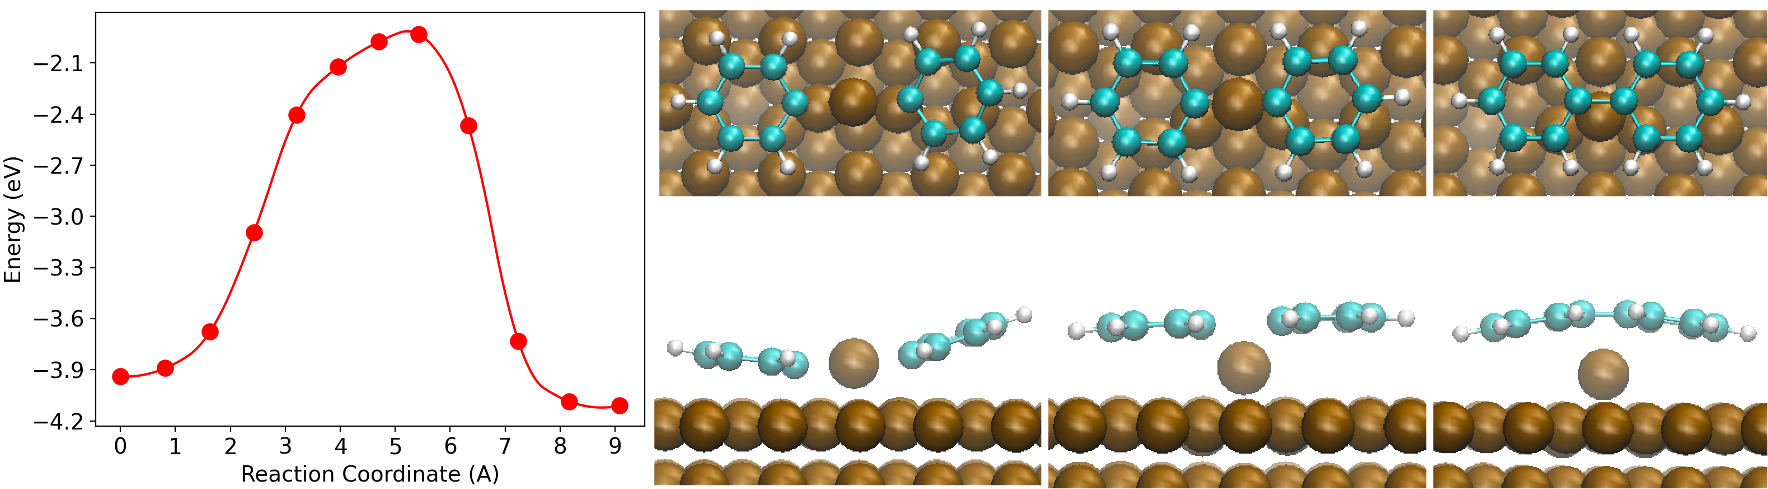
\includegraphics[width=1.0\textwidth]{Fig/bondformadatom.png}
\caption{C-C bond formation through new formed adatom Path II}
\label{fig:bondformadatom}
\end{figure*}

%R1111: All titles and subtitles use sentence case, meaning only the first word is capitalized.
\subsubsection{Path I vs path II}

Taking the data of Path I and Path II into consideration, finally, a feasible C--C bond was constructed in both cases (bond length is around 1.5 \AA\, expected to be 1.34 \AA\ - 1.54 \AA). From thermodynamic aspect, Path I is much more exothermic, which means it will lead to a more stable product. Kinetically, the activation energy of Path I is also smaller than Path II, which means at the same temperature, the Path I reaction would take place at a higher speed and account for a much larger percentage. In this case, we could safely conclude that, if there is no pre-exiting adatom on copper surface, the formation of C--C bond in surface Ullmann coupling will follow the path I.

%R1111: Compare C--C distance in IM4 and IM5 to the experimental data for Ph-Halogen. Can we see IM5 experimentally? 3.89Ang vs 3.1Ang.


%R1111: Note that the difference between dimer1 and dimer2 is smaller than the difference between FS1 and IS. Probably because the dimer interacts stronger with the adatom than with the surface. 


\subsection{Energy diagram of complete Surface Ullmann Coupling Reaction}

In this section, the summary of thermodynamic data of all intermediates in surface Ullmann coupling reaction is present in one diagram. As is shown in Fig.~\ref{fig:completeenergy}.

Here taking the surface Ullmann coupling between two bromobenzene as example, the physisorption of two bromobenzene on Cu(111) surface decrease the energy of the whole system by 2.35 eV, which is widely recognized in experiment because adsorbing aromatic species on copper surface as a fast procedure. 
Then till the formation of new C--C bond, a detailed discussion has been demonstrated in previous sections. The last two successive steps are concerned with the desorption of biphenyl molecule and two dehalogenated bromine atoms. 
In total, the red line is more energetically favourable than green line, that can be considered to be a more reasonable pathway in realistic surface Ullmann coupling if there is no pre-exiting adatom on metal surface.

%%% Early steps
%R1111: LATER. Do we need adatom calculations for TS1? Perhaps only one or two halogen-metal pairs (for complete diagram). How will it affect the subsequent steps? Will the PH-Adatom roam the surface together before encountering the second Ph? PRIORITY6.
%R1111: Why there is no Cu-atom lifting during the C-X bond dissociation? Compare to previous works. Actually partial lifting is a process with a barrier for Au and Ag surfaces but not for Cu. We might need to reproduce this after all. --> More comparison to the existing calculation is required.

%%% Late steps
%R1111: Is the later part of the diagram halogen independent? YES!
%R1111: The barrier between IM4 and IM5 is important. Because it seems that it exists when the adatom is pulled by the R-X dissociation. PRIORITY2. Use NEB to find it.
%R1111: We need free energy for the important IM4->IM5 step. This will include increased entropy of the adatom-vacancy system (assuming that the atom with two phenyls diffuse freely). PRIORITY4.
%R1111: What is the energy of the state after dimer1, when the dimer "falls" flat to the surface? It should be around -3.97 eV. dimer1-2: dimer2+fs1-IS-IS=-3.97 eV
%R1111: An alternative TS2-1 must be calculated. The final product should be lying flat on the surface. PRIORITY3.
%R1111: What effect is responsible for the energy lowering upon adatom creation in IM5? Note that for I--Ph on Cu the extraction+diffusion during the C-I breaking step produces the overall uphill step. PRIORITY1. Remove Ph in IM3, IM4, IM without geometry relaxation (only the metal surface, not phenyl).

%%% Minor comments
%R1111: State labeling is poorly planned. Relabel states to stick to one system.
%R1111: Should we add one more TS between IM2 and IM3? LATER.
%R1111: How does the vacancy affect the energy? LATER.
%R1111: Halogen filling the vacancy or sitting on top of the adatom? PRIORITY5.

%RZK1222: This important effect needs to be properly described. The height of TS2-1 means that IM5, once formed will not undergo the C--C bond formation and can be viewed as an undesirable by-product of the reaction (unless it exists in quick equilibrium with IM4, which can be entropically hindered -- hard to find that vacancy again).

%RZK1222: How difficult is it to push the adatom (with attached organic radicals) DOWN?

\begin{figure*}[hbt]
\centering
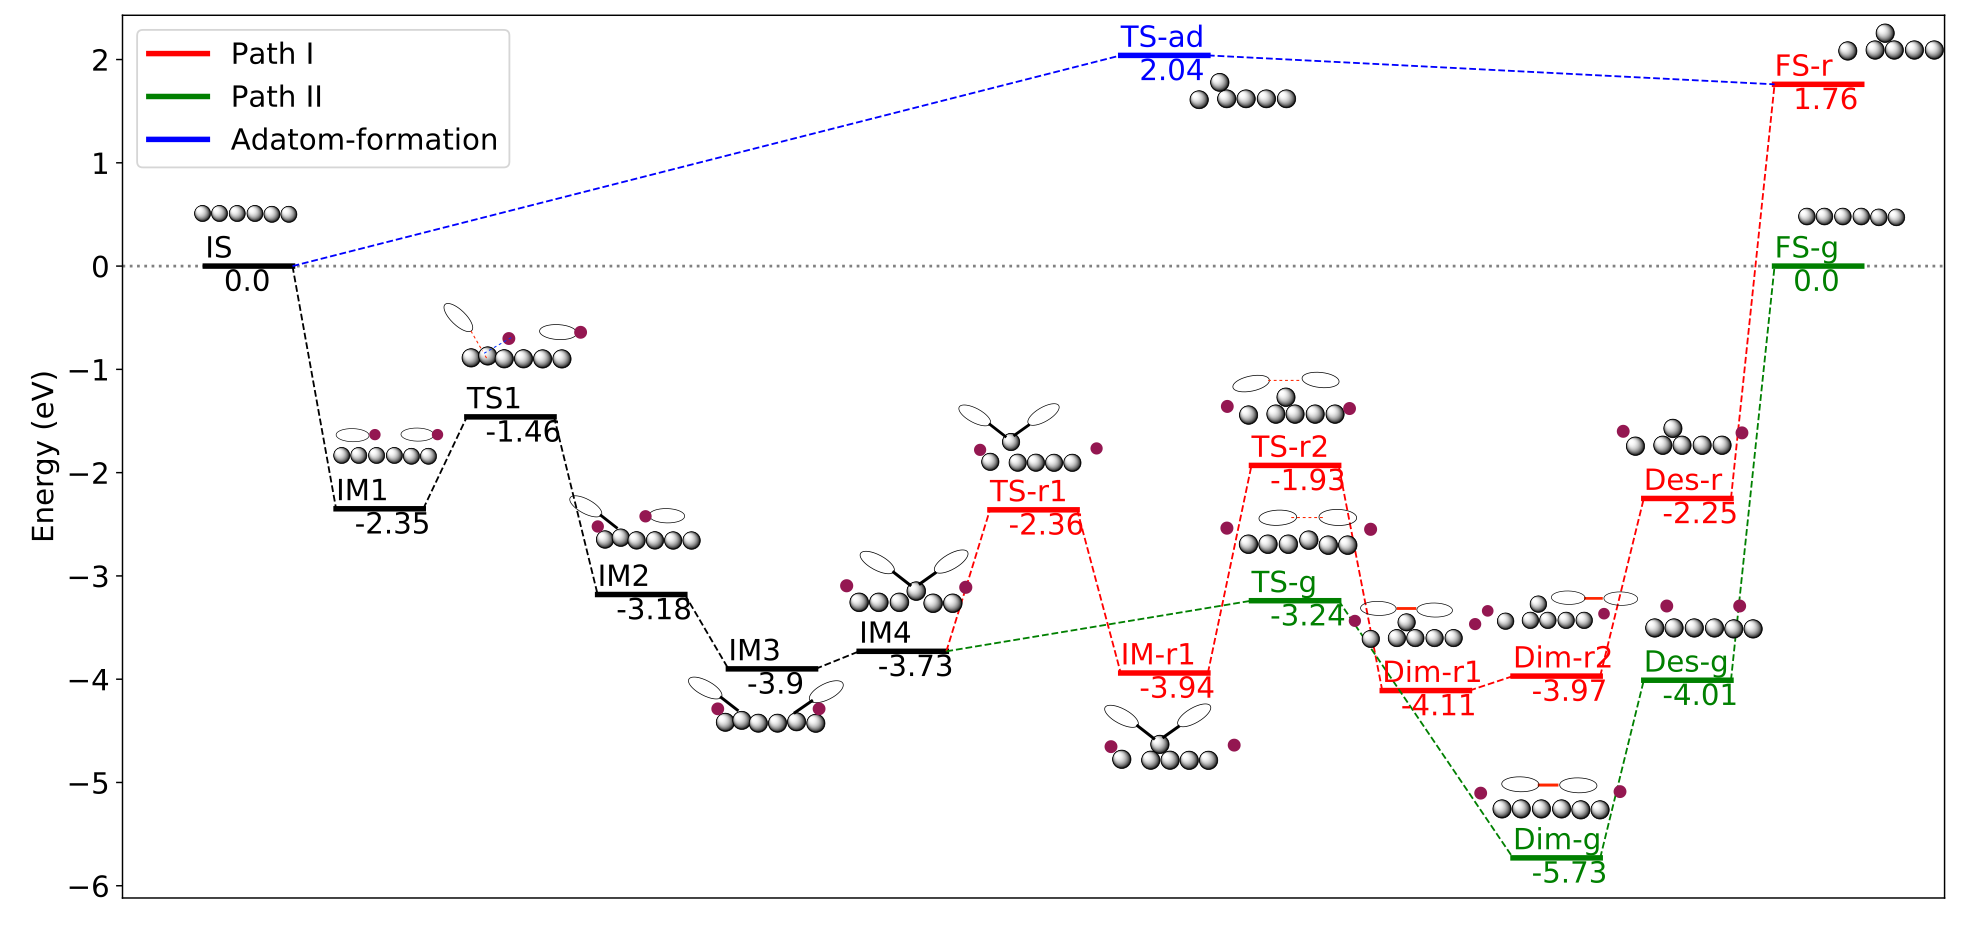
\includegraphics[width=0.98\textwidth]{Fig/completeenergy.png}
\caption{The Energy Diagram of Surface Ullmann Coupling Reaction.
the red line is the surface Ullmann Coupling reaction following Path II, the green line is following Path I. Finally, red line ended with a adatom-vacancy pair on Cu(111) surface and the green line ended same as the original Cu(111) surface.(red circle means bromine atoms)}
\label{fig:completeenergy}
\end{figure*}

\subsection{Formation of Adatom on Pure Cu Surface}

Finally, the energy of forming an adatom on a perfect Cu(111) surface is also presented. The goal of showing this energy diagram is to launch a comparison between two different conditions, both of which deliver an adatom on Cu(111) surface. One is the formation without any species on metal surface, the other one is with surface Ullmann coupling reaction.
As Figure.~\ref{fig:pureadatomform} shows, the reaction of forming a new adatom-vacancy pair on perfect Cu(111) surface is endothermic, $\Delta H$ is 1.76 eV and the $E_{barrier}$ is 2 eV. This means at room temperature, the formation of adatom is unfavourable. 
However, as is shown in Fig.~\ref{fig:completeenergy}, the presence of organometallic intermediate in surface Ullmann coupling could promote the formation of adatoms on surface both thermodynamically and kinetically. This pathway might be considered as a plausible method to create adatoms on metal surface.

\begin{figure*}[hbt]
\centering
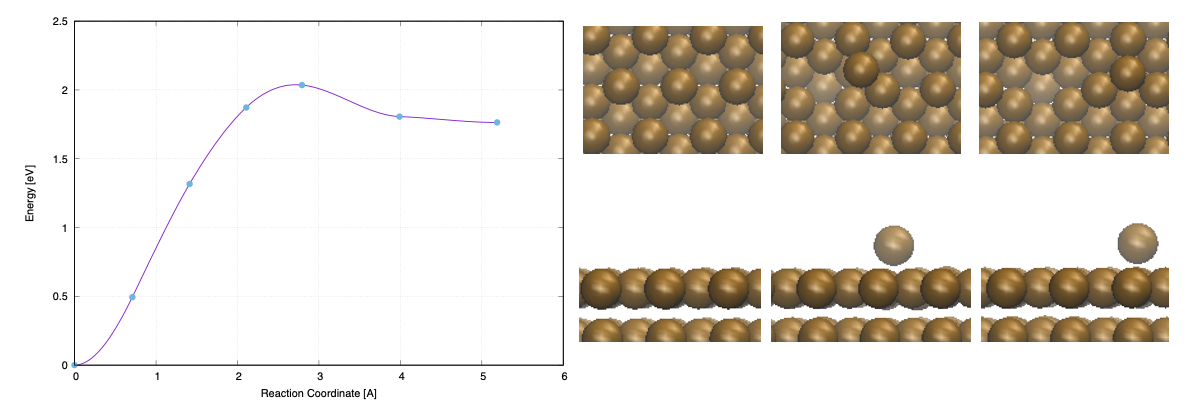
\includegraphics[width=1.0\textwidth]{Fig/pureadatomform.png}
\caption{adatom formation on pure Cu(111) surface}
\label{fig:pureadatomform}
\end{figure*}

\section{conclusions}

\section{acknowledgements}

\section{Articles to read}

\href{https://doi.org/10.1016/j.apsusc.2020.145797}{Ullmann coupling of 2,7-dibromopyrene on Au(1 1 1) assisted by surface adatoms}

\nocite{*}

\bibliographystyle{apsrev4-1} % Tell bibtex which bibliography style to use
\bibliography{references}% Produces the bibliography via BibTeX.

\end{document}
